\chapter{Deep Learning}
\section{Einleitung}
Künstliche neuronale Netze stellen eine Klasse von Modellen des maschinellen Lernens dar, die vom Zentralnervensystem von Säugetieren inspiriert sind. Jedes Netz besteht aus mehreren miteinander verbundenen \enquote{Neuronen}, die in \enquote{Schichten} organisiert sind. Neuronen in einer Schicht leiten Nachrichten an Neuronen in der nächsten Schicht weiter. Erste Studien wurden in den frühen 50er Jahren mit der Einführung des \enquote{Perzeptrons} \cite{Rosenblatt} begonnen, eines zweischichtigen Netzwerks, das für einfache Operationen verwendet wird, und in den späten 60er Jahren mit der Einführung des \enquote{Back-Propagation-Algorithmus} (effizientes mehrschichtiges Netzwerktraining) (gemäß \cite{Werbos1990}, \cite{Hinton}) weiter ausgebaut.

Deep Learning ermöglicht es Computermodellen, die aus mehreren Verarbeitungsebenen bestehen, Darstellungen von Daten mit mehreren Abstraktionsebenen zu erlernen. Diese Verfahren haben den Stand der Technik in Bezug auf Spracherkennung, visuelle Objekterkennung, Objekterkennung und viele andere Bereiche wie die Genomik dramatisch verbessert. Deep Learning entdeckt komplexe Strukturen in großen Datenmengen, indem es den Backpropagation-Algorithmus verwendet. Dieses ist ein Verfahren, welches der Maschine zeigt, wie sie ihre internen Parameter ändern soll, mit denen die Darstellung in jeder Schicht aus der Darstellung in der vorherigen Schicht berechnet wird. Tiefe Faltungsnetze haben Durchbrüche bei der Verarbeitung von Bildern, Video, Sprache und Audio gebracht, während wiederkehrende Netze sequentielle Daten wie Text und Sprache beleuchtet haben \cite*{Lecun2015}.


\section{Überwachtes Lernen}


Die häufigste Form des maschinellen Lernens, ob tief oder nicht, ist das überwachte Lernen. Beim überwachten Lernen werden zunächst große Mengen an Daten gesammelt, die jeweils mit ihrer Kategorie gekennzeichnet sind. Währen des Trainings wird der Maschine ein Exemplar aus den Daten gezeigt und es wird eine Ausgabe in Form eines Bewertungsvektors erzeugt, einer für jede Kategorie. Der Wunsch ist es, für jede Kategorie die höchste Punktzahl zu erreichen. Es wird eine Zielfunktion berechnet, die den Fehler (oder Abstand) zwischen den Ausgabewerten und dem gewünschten Bewertungsmustern misst. Die Maschine ändert dann ihre internen einstellbaren Parameter um, um den Fehler zu minimieren. Diese einstellbaren Parameter werden \textbf{Gewichte} genannt. Gewichte sind reelle Zahlen die als \enquote{Knöpfe} gesehen werden können, die die Eingabe-Ausgabe-Funktion der Maschine ist. In einem typischen Deep-Learning-System können Hunderte Millionen dieser einstellbaren Gewichte vorkommen \cite*{Lecun2015}. Neben den Gewichten taucht der Begriff \textbf{Bias} auf, welches im Deep Learning ein Maß dafür ist, das Perzeptron zum \enquote{feuern zu bringen} \cite*[7]{Nielsen2015}.


\section{Das Perzeptron}
Das Perzeptron ist ein einfacher Algorithmus mit einem Eingabevektor $x$ mit $m$ Werten $(x_2, ..., x_m)$. Es wird oft als \enquote{Eingabe-Features} oder einfach als \enquote{Features} bezeichnet. Es gibt entweder eine $1$ \enquote{Ja} oder eine $0$ \enquote{Nein} zurück (siehe Formel~\ref{Formel2_1}). Dabei ist $w$ ein Vektor welches das Gewicht darstellt, und $wx$ das Punktprodukt aus $\begin{array}{l}
        {\textstyle \sum ^{m}_{j=1}} w_{j} x_{j} \\
    \end{array}$, $b$ ist der Bias. Aus $wx + b$ ist die Grenzhyperebene definiert, die die Position gemäß den $w$ und $b$ zugewiesenen Werten ändert.

\begin{equation}
    fx=\begin{cases}
        1 & wx+b >0   \\
        0 & ansonsten
    \end{cases}
    \label{Formel2_1}
\end{equation}

Beispielsweise kann das Perzeptron bei drei Eingabemerkmalen  (Rot, Grün und Blau) unterscheiden, ob die Farbe weiß ist oder nicht. Es soll beachtet werden, dass das Perzeptron keine \enquote{Vielleicht}-Antwort ausdrücken kann. Es kann mit \enquote{Ja} (1) oder \enquote{Nein} (0) antworten. Das Perzeptron-Modell kann dafür verwendet werden, indem durch Anpassung von $w$ und $b$, das Modell trainiert wird.



\section{Mehrschichtiges Perzeptron}

Wenn ein Modell nicht nur eine einzige lineare Schicht hat, sondern wenn mehrere Schichten in Form von Perzeptronen zusammengebracht werden, handelt es sich dabei um ein mehrschichtiges Perzeptron. Die Eingabe- und Ausgabeebene  ist von außen sichtbar, während alle anderen Ebenen in der Mitte ausgeblendet oder verborgen sind (hidden layers). Es werden mehrere lineare Funktionen (einzelne Schichten) nacheinander gestapelt und somit eine  mehrschichtiges Perzeptron erzeugt.

\begin{figure}[H]
    \centering
    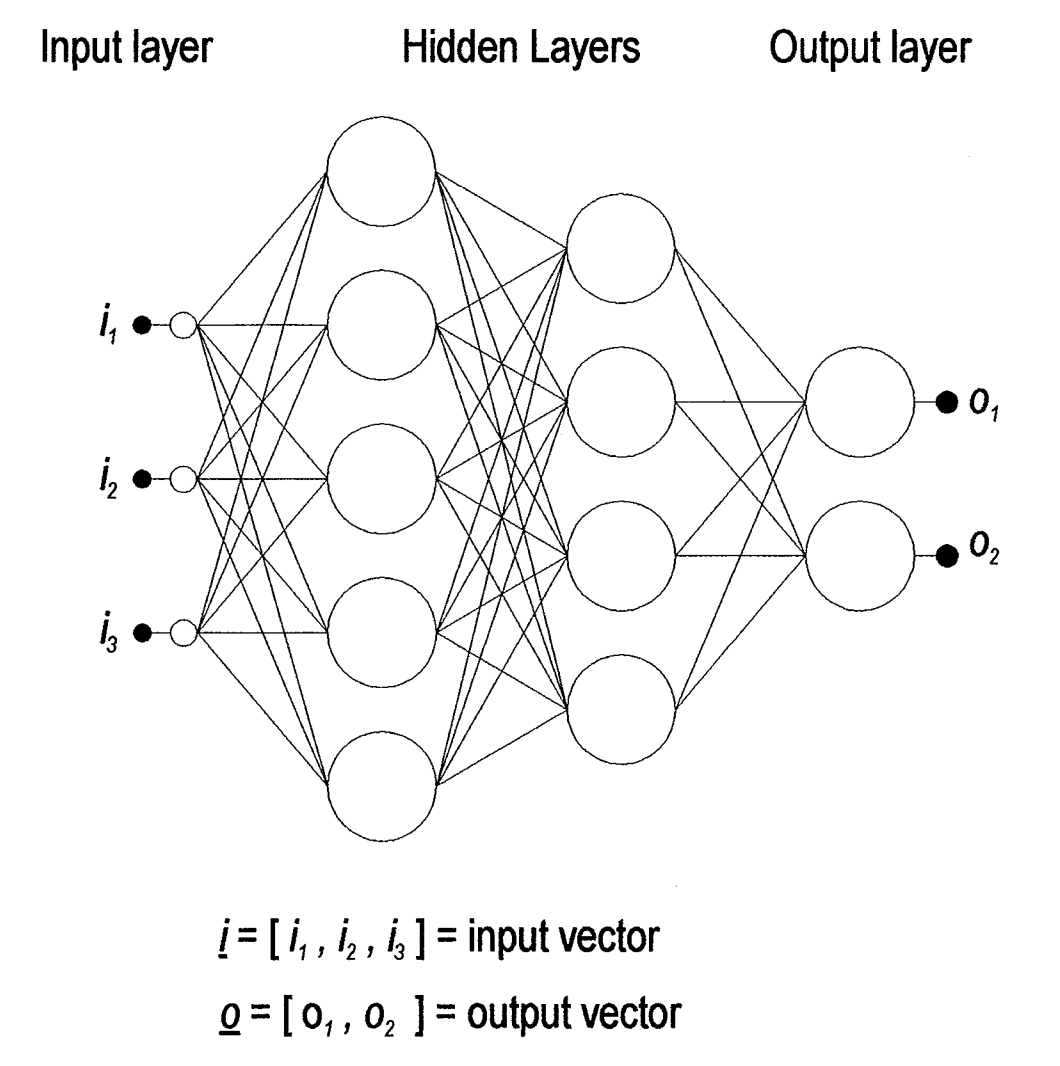
\includegraphics[width=8cm]{kapitel2/multilayerperc.png}
    \caption[Das mehrschichtige Perzeptron]{Das mehrschichtige Perzeptron mit zwei verborgenen Schichten, entnommen aus \cite*{Gardner1998}}
    \label{Kap2:Multi}
\end{figure}


\section{Sigmoid-Neuron}

Neben dem Perzeptron gibt es das Sigmoid Neuron. Das Perzeptron gibt bekannt nur eine 0 oder eine 1 zurück. Es ist also eine Funktion nötig, die sich ohne ohne Diskontinuität schrittweise von 0 auf 1 ändert. Mathematisch bedeutet dies, dass eine stetige Funktion nötig ist, mit der die Ableitung berechnet werden kann. Dieses Problem kann überwunden werden, indem einen neuer Typ eines künstlichen Neurons eingeführt wird, der als \textbf{Sigmoid-Neuron} bezeichnet wird. Sigmoid Neuronen ähneln Perzeptronen, sind jedoch so modifiziert, dass kleine Änderungen ihres Gewichts und ihres Bias nur eine geringe Änderung ihrer Leistung bewirken. Dies ist der Grund dafür, dass Netzwerke lernen können \cite*[8]{Nielsen2015}.


Genau wie ein Perzeptron hat das Sigmoid-Neuron die Eingaben $x_1, x_2, ...$, aber anstatt nur 0 oder 1 zu sein, können diese Eingänge auch beliebige Werte zwischen 0 und 1 annehmen. Also zum Beispiel 0,123 welches eine gültige Eingabe für ein Sigmoid-Neuron ist. Ebenso wie ein Perzeptron hat das Sigmoid-Neuron Gewichte für jede Eingabe, $w_1, w_2, ...$ und einen Bias, $b$. Die Ausgabe ist jedoch nicht 0 oder 1, stattdessen ist es $\sigma$, $(wx + b)$, wobei $\sigma$ als Sigmoidfunktion bezeichnet wird und durch Formel~\ref{Formel2_2} definiert ist.

\begin{equation} \label{Formel2_2}
    \sigma (z) = \frac{1}{1+e^{-z}}
\end{equation}


\section{Aktivierungsfunktionen}
Ohne eine \textbf{Aktivierungsfunktion} (auch als Nichtlinearität bezeichnet) würde die dichte Schicht (dense layer) nur aus zwei linearen Operationen bestehen - einem Punktprodukt und einer Addition: $Ausgabe = Punkt (w, Eingabe) + b$. Die Schicht konnte also nur lineare Transformationen (affine Transformationen) der Eingabedaten lernen. Um Zugang zu einem viel umfangreicheren Hypothesenraum zu erhalten, wird eine Nichtlinearitäts- oder Aktivierungsfunktion benötigt \cite*[S. 72]{Chollet2017}.

\subsection{Sigmoid}
Die Sigmoidfunktion wird mit der Formel~\ref{Formel2_2} definiert und in der Abbildung~\ref{Kap2:Sigmoid_plot} dargestellt, die Ableitung der Sigmoidfunktion wird in der Formel~\ref{Formel2_2Abl} definiert. Sie hat kleine Ausgangsänderungen im Bereich (0, 1), wenn der Eingang im Bereich $(-\infty, \infty)$ variiert. Mathematisch ist die Funktion stetig. Ein Neuron kann das Sigmoid zur Berechnung der nichtlinearen Funktion $\sigma(z = wx + b)$ verwenden. Wenn $z = wx + b$ sehr groß und positiv wird, dann wird $e^z \rightarrow 0$ also $\sigma(z) \rightarrow 1$, während wenn $z = wx + b$ sehr groß und negativ wird, wird $e^{-z} \rightarrow 0$ also $\sigma(z) \rightarrow 0$. Mit anderen Worten, ein Neuron mit Sigmoidaktivierung hat ein ähnliches Verhalten wie das Perzeptron, aber die Änderungen sind allmählich und Ausgabewerte wie 0,54321 oder 0,12345 sind vollkommen legitim. In diesem Sinne kann ein Sigmoid-Neuron auch mit \enquote{vielleicht} antworten \cite*[10]{AntonioGuili;AmitaKapoor;SujitPal2019}.

\begin{figure}[H]
    \centering
    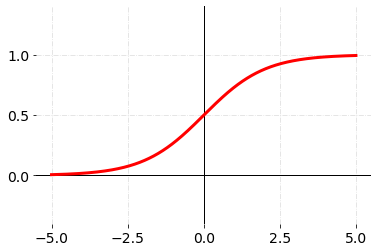
\includegraphics[width=8cm]{kapitel2/sig_plot.png}
    \caption[Darstellung der Sigmoid-Aktivierungsfunktion]{Darstellung der Sigmoid-Aktivierungsfunktion (eigene Darstellung)}
    \label{Kap2:Sigmoid_plot}
\end{figure}


\begin{equation} \label{Formel2_2Abl}
    \begin{array}{ c }
        \sigma '(z)\ =\ \frac{d}{dz}\left(\frac{1}{1+e^{-z}}\right) =\frac{1}{\left( 1+e^{-z}\right)^{-2}}\frac{d}{dz} =\left( e^{-z}\right) \ =\frac{e^{-z}}{\left( 1+e^{-z}\right)}\frac{1}{\left( 1+e^{-z}\right)} \ =  \\
        \\
        \frac{e^{-z} +1-1}{\left( 1+e^{-z}\right)}\frac{1}{\left( 1+e^{-z}\right)} =\left(\frac{\left( 1+e^{-z}\right)}{\left( 1+e^{-z}\right)} -\frac{1}{\left( 1+e^{-z}\right)}\right)\frac{1}{\left( 1+e^{-z}\right)} = \\
        \\
        \left( 1-\frac{1}{\left( 1+e^{-z}\right)}\right)\left(\frac{1}{\left( 1+e^{-z}\right)}\right) =\ (1-\sigma (z))\sigma (z)
    \end{array}
\end{equation}

\subsection{Tanh}
Die Tanh-Aktivierungsfunktion wird mit der Formel~\ref{Formel2_3} definiert ihre Ableitung wird in der Formel~\ref{Formel2_3Abl} berechnet. Sie hat ihre Ausgangsänderungen im Bereich (-1, 1). Sie hat eine Struktur, die der Sigmoid-Funktion sehr ähnlich ist. Der Vorteil gegenüber der Sigmoidfunktion besteht darin, dass ihre Ableitung steiler ist, was bedeutet, dass sie mehr Werte enthalten kann (vergleiche Abbildung~\ref{Kap2:Tanh_plot}). Für die Ableitung der Tanh-Aktivierungsfunktion gilt, $e^z = \frac{d}{dz}e^z$ und $e^{-z} = \frac{d}{dz}e^{-z}$.

\begin{equation} \label{Formel2_3}
    tanh(z) = \frac{e^{z}-e^{-z}}{e^{z}-e^{-z}}
\end{equation}

\begin{equation} \label{Formel2_3Abl}
    \begin{array}{ c }
        \frac{d}{dz} tanh( x) =\frac{\left( e^{z} +e^{-z}\right)\left( e^{z} +e^{-z}\right) -\left( e^{z} -e^{-z}\right)\left( e^{z} -e^{-z}\right)}{\left( e^{z} +e^{-z}\right)^{2}} = \\
        \\
        1-\frac{\left( e^{z} -e^{-z}\right)^{2}}{\left( e^{z} +e^{-z}\right)^{2}} \ =\ 1\ -tanh^{2}( z)
    \end{array}
\end{equation}

\begin{figure}[H]
    \centering
    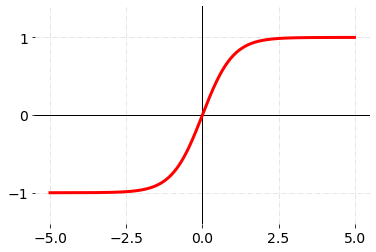
\includegraphics[width=8cm]{kapitel2/tanh_plot.png}
    \caption[Darstellung der Tanh-Aktivierungsfunktion]{Darstellung der Tanh-Aktivierungsfunktion (eigene Darstellung)}
    \label{Kap2:Tanh_plot}
\end{figure}

\subsection{ReLu}
Vor kurzem wurde eine sehr einfache Funktion namens ReLU (REctified Linear Unit) sehr beliebt, da sie dazu beiträgt, einige Optimierungsprobleme die bei Sigmoiden beobachtet werden, zu lösen \cite*[11]{AntonioGuili;AmitaKapoor;SujitPal2019}. Sie wird in Formel~\ref{Formel2_4} definiert, die zugehörige Ableitungsfunktion wird in der Formel~\ref{Formel2_4Abl} berechnet. Wie in Abbildung~\ref{Kap2:ReLu_plot} zu sehen, ist die Funktion für negative Werte Null und wächst für positive Werte linear. Die ReLU ist relativ einfach zu implementieren.

\begin{equation} \label{Formel2_4}
    f( x) \ =\ \begin{cases}
        0 & wenn\ x\  <\ 0    \\
        x & wenn\ x\  \geq\ 0 \\
    \end{cases}
\end{equation}

\begin{equation} \label{Formel2_4Abl}
    f'( x) \ =\ \begin{cases}
        1, & wenn\ x\  >\ 0 \\
        0, & sonst
    \end{cases}
\end{equation}

\begin{figure}[H]
    \centering
    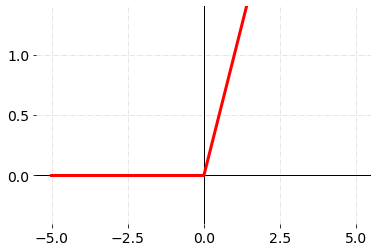
\includegraphics[width=8cm]{kapitel2/relu_plot.png}
    \caption[Darstellung der ReLu-Aktivierungsfunktion]{Darstellung der ReLu-Aktivierungsfunktion (eigene Darstellung)}
    \label{Kap2:ReLu_plot}
\end{figure}

\subsection{softmax}
Die grundlegende Schwierigkeit bei der Durchführung kontinuierlicher Mathematik auf einem digitalen Computer besteht darin, dass unendlich viele reelle Zahlen mit einer endlichen Anzahl von Bitmustern dargestellt werden müssen. Dabei entstehen Rundungsfehler die problematisch sein können, insbesondere wenn sie sich über viele Operationen hinweg zusammensetzen. Sieführen dazu, dass theoretisch funktionierende Algorithmen in der Praxis fehlschlagen. Ein Beispiel für eine Funktion, die gegen Rundungsfehler stabilisiert, ist die softmax-Funktion \cite*[80-81]{IanGoodfellowYoshuaBengio2016}.

\begin{equation} \label{FormelSoft}
    softmax( x)_{i} =\frac{exp( x_{i})}{\sum ^{n}_{j=1} exp( x_{j})}
\end{equation}

\section{Optimierungsalgorithmen}
Die meisten Deep-Learning-Algorithmen beinhalten irgendeine Art von Optimierung. Optimierung bezieht sich auf die Aufgabe, eine Funktion $f(x)$ durch Ändern von $x$ entweder zu minimieren oder zu maximieren. Die meisten Optimierungsprobleme werden in Bezug auf Minimierung von $f(x)$ formuliert. Die Maximierung kann über einen Minimierungsalgorithmus durch Minimieren von $-$$f(x)$ erreicht werden. Die Funktion die minimiert oder maximiert werden soll, wird als \textbf{Objektive Funktion} bezeichnet. Es wird auch \textbf{Kostenfunktion} oder \textbf{Verlustfunktion} bezeichnet. Zum Beispiel ist die Funktion $x^{*} = arg\ min\ f( x)$ eine solche Funktion.

        \subsection{Gradientenverfahren}
        Der Gradientenabstieg ist einer der beliebtesten Algorithmen zur Optimierung und bei weitem der häufigste Weg zur Optimierung neuronaler Netze. Der Gradientenabstieg ist ein Weg, um eine Zielfunktion $J(\theta)$ zu minimieren, die durch die Parameter eines Modells $\theta \in \mathbb{R}^{d}$ parametrisiert wird. Die Parameter werden in der entgegengesetzten Richtung des Gradienten der Zielfunktion $\nabla \theta J (\theta)$ angepasst. Die Lernrate $\eta$ bestimmt die Größe der Schritte, die unternommen werden, um ein lokales Minimus zu erreichen. Mit anderen Worten, wird der Richtung bergab gefolgt, die durch die Zielfunktion erzeugt wird, bis ein \enquote{Tal} erreicht wird (siehe Abbildung~\ref{Kap2:Grad}) \cite*{Ruder2016}.



        \begin{figure}[H]
            \centering
            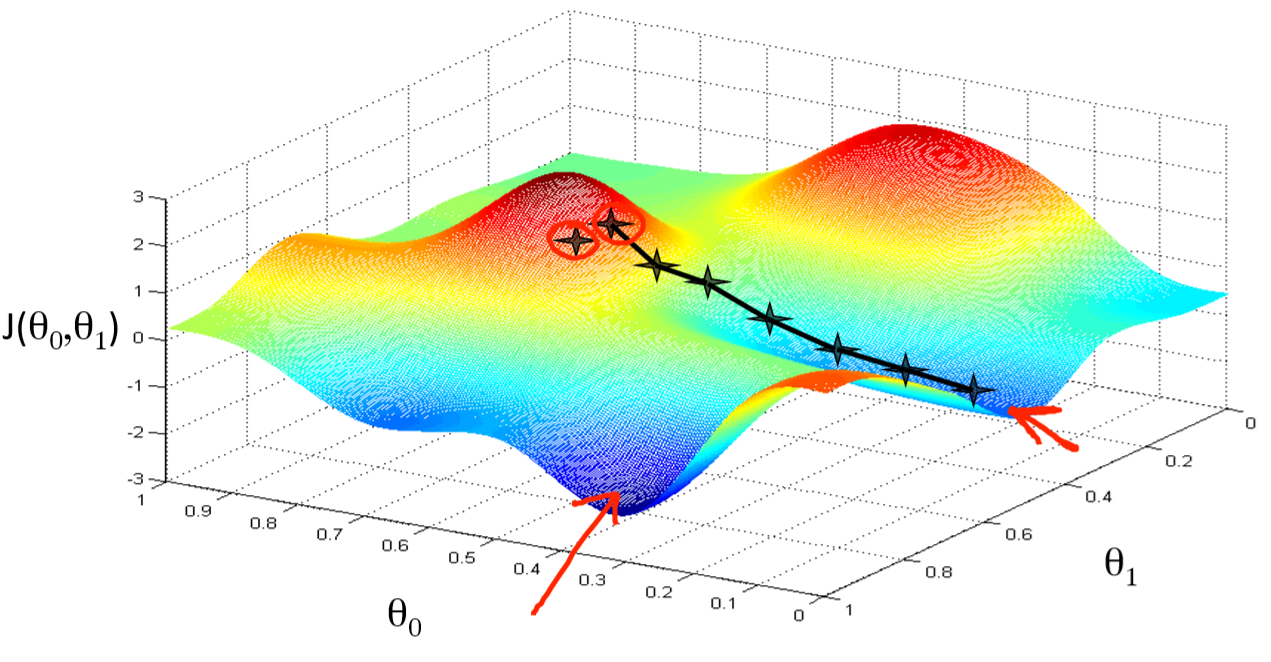
\includegraphics[width=12cm]{kapitel2/gradient.png}
            \caption[Der Gradientenabstieg]{Darstellung des Gradientenabstiegs, entnommen aus \cite*{hackernoon}.}
            \label{Kap2:Grad}
        \end{figure}



        \subsection{Batch Gradientenabstiegsverfahren}
        Der Standart Gradientenabstiegsverfahren, auch Batch Gradientenabstiegsverfahren genannt, berechnet den Gradienten der Verlustfunktion zu den Parametern $\theta$ für den gesamten Trainingsdatensatz.


        \begin{equation} \label{FormelGradBatch}
            \theta = \theta - \eta \cdot \nabla_{\theta}J(\theta)
        \end{equation}

        Da der gesamte Datensatz berechnet werden muss, um nur eine Aktualisierung durchzuführen, kann der Batch Gradientenabstieg sehr langsam sein und ist für Datensätze, die nicht in den Speicher passen, nicht zu handhaben. Der Batch Gradientenabstieg ermöglicht es auch nicht, das Modell mit neuen Beispielen im laufenden Betrieb zu aktualisieren \cite*{Ruder2016}.

        \subsection{Stochastische Gradientenabstiegsverfahren}

        Im Gegensatz dazu führt der stochastische Gradientenabstiegsverfahren (SGD) eine Parameteraktualisierung für jedes Trainingsbeispiel durch. Der Batch Gradientenabstieg führt redundante Berechnungen für große Datenmengen durch, da Gradienten für ähnliche Beispiele vor jeder Parameteraktualisierung neu berechnet werden. Der Stochastische Gradientenabstiegsverfahren beseitigt diese Redundanz, indem jeweils ein Update durchgeführt wird. Es ist daher in der Regel viel schneller und kann auch beim laufendem Lernen verwendet werden \cite*{Ruder2016}.

        \begin{equation} \label{FormelGradStoch}
            \theta = \theta - \eta \cdot \nabla_{\theta}J(\theta;x^{(i)};y^{(i)})
        \end{equation}



        \section{Backpropagation}
        Das \textbf{Backpropagation} Verfahren bezieht sich auf die Gewichte eines mehrschichtigen Netzes und wendet dabei praktisch die Anwendung der Kettenregel der  Differentialrechnung an. Es wird vom Gradienten in Bezug auf die Ausgabe (oder die Eingabe der Nachfolge) rückwärts gearbeitet. Die Kettenregel sagt dabei aus, wie zwei kleine Effekte (eine kleine Änderung von $x$ auf $y$ und der von $y$ auf $z$) zusammengesetzt sind. Eine kleine Änderung von $\Delta y$ in $x$ wird zuerst in eine kleine Änderung $\Delta y$ in $y$ umgewandelt, indem sie mit $\frac{\partial y}{\partial y}$  multipliziert wird (die partielle Ableitung). In ähnlicher Weise erzeugt die Änderung $\Delta y$ eine Änderung von $\Delta z$ in $z$ (siehe Formel~\ref{ChainRule}) \cite*{Lecun2015}.

        \begin{gather} \label{ChainRule}
            \Delta z =  \frac{\partial z}{\partial y} \Delta y \notag\\
            \Delta y = \frac{\partial y}{\partial x} \Delta x \notag\\
            \Delta z = \frac{\partial z}{\partial y}\frac{\partial y}{\partial x} \Delta x \notag\\
            \frac{\partial z}{\partial x} = \frac{\partial z}{\partial y} \frac{\partial y}{\partial x}
        \end{gather}




        Die Gleichungen, die zur Berechnung des \textbf{Vorwärtsdurchlaufs} (siehe Abbildung~\ref{BackProp}) in einem neuronalen Netz mit zwei verborgenen Schichten und einer Ausgangsschicht verwendet werden, bilden jeweils ein Modul, durch das man Gradienten zurückpropagieren kann. Auf jeder Ebene wird zuerst die Gesamteingabe $z$ für jede Einheit berechnet. Dann wird eine nichtlineare Funktion auf $z$ angewendet, um die Ausgabe der Einheiten zu erhalten (der Bias wurde hier der Einfachheit halber weggelassen). Eine nichtlineare Funktion kann z.B. eine ReLu- oder eine Sigmoid-Funktion oder eine tanh-Funktion sein. Im \textbf{Rückwärtsdurchlauf} (siehe Abbildung~\ref{BackProp}) wird in jeder verborgenen Schicht die Fehlerableitung in Bezug auf die Ausgabe jeder Einheit berechnet. Dies geschieht durch Vergleichen der Ausgaben mit der richtigen Antwort, um Fehlerableitungen zu erhalten \cite*{Lecun2015}.


        \begin{figure}[H]
            \centering
            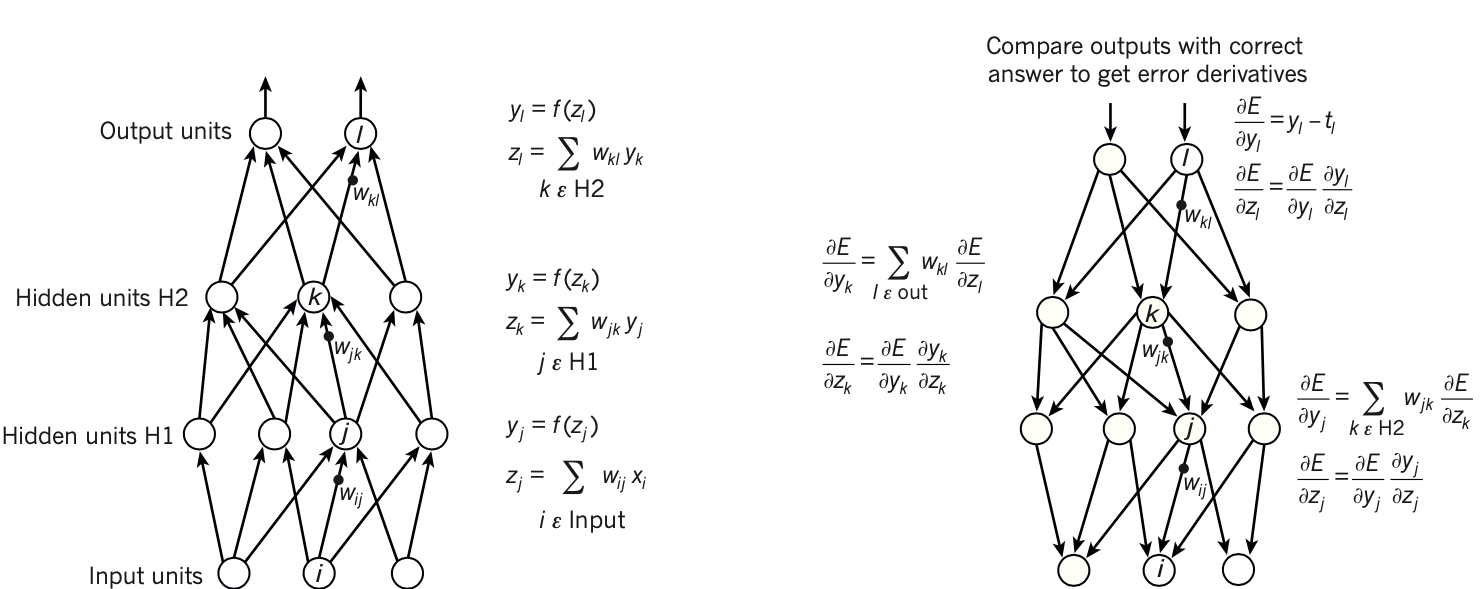
\includegraphics[width=13cm]{kapitel2/backprop.png}
            \caption[Die Vorwärts- und Rückwärtsschritte im Backpropagation]{Darstellung vergleicht die Schritte des Backpropagation Verfahrens nach vorne und hinten (in Anlehnung an \cite*{Lecun2015}).}
            \label{BackProp}
        \end{figure}

        Die Backpropagation-Gleichung wird wiederholt angewendet. Der Rückwärtsdurchlauf bezieht sich auf die Idee, die Differenz zwischen Vorhersage- und Istwerten zu verwenden, um die Hyperparameter der verwendeten Methode anzupassen. Für die Anwendung ist jedoch immer eine vorherige Vorwärtspropagation erforderlich.


        \section{Lernrate im Deep Learning}
        Die \textbf{Lernrate} beeinflusst den Betrag, um den die Parameter während der Optimierung angepasst werden, um den Fehler des neuronalen Netzwerks zu minimieren. Es ist ein Koeffizient, der die Größe der Schritte (Aktualisierungen) skaliert, die ein neuronales Netzwerk auf seinen Parameter (Vektor $x$) ausführt, wenn es den Verlustfunktionsraum durchquert. Ein großer Lernratenkoeffizient (z. B. 1) lässt die Parameter Sprünge machen, und kleine (z. B. 0,00001) lassen ihn langsam voranschreiten. Im Gegensatz dazu sollten kleine Lernraten letztendlich zu einem Fehlerminimum führen (es kann eher ein lokales als ein globales Minimum sein). Sehr kleine Lernraten können sehr lange dauern und die Belastung eines bereits rechenintensiven Prozesses erhöhen  \cite*[77]{Patterson2019}.


        \begin{figure}[H]
            \centering
            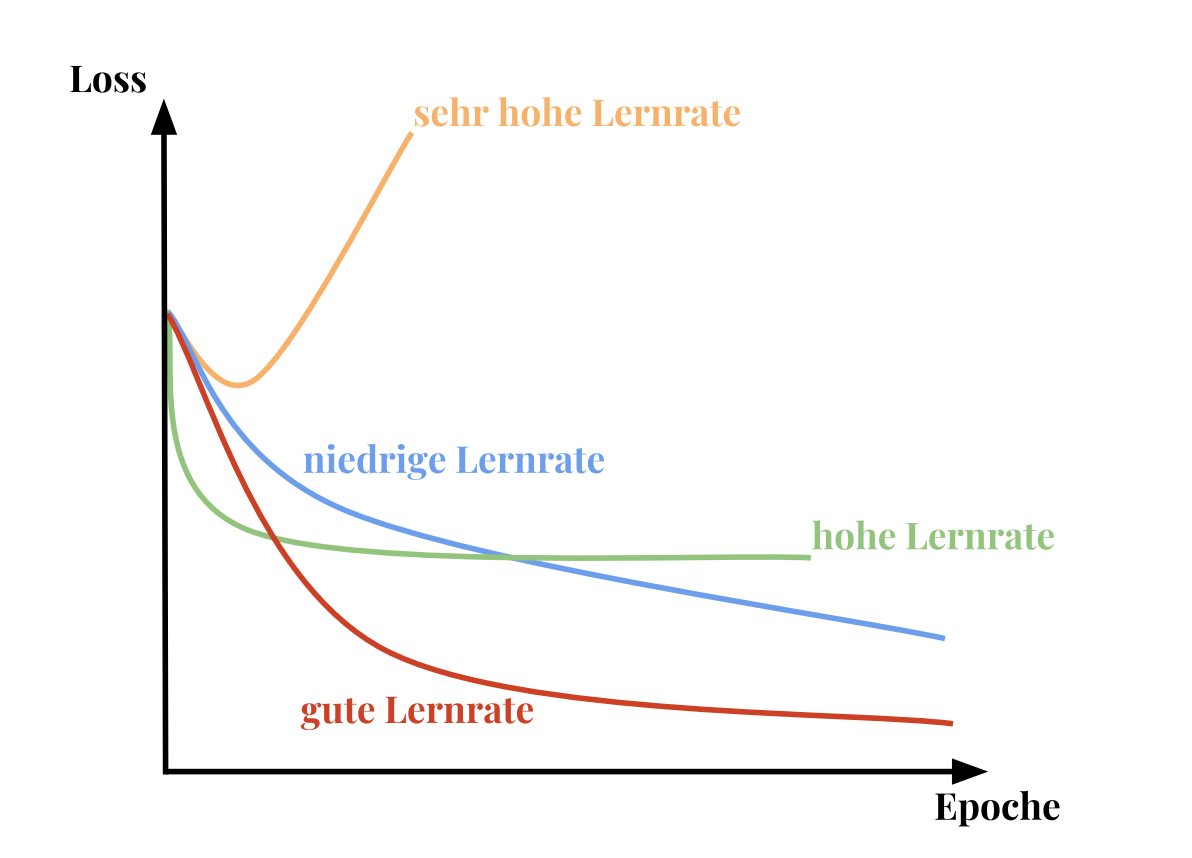
\includegraphics[width=10cm]{kapitel2/learnrate.png}
            \caption[Einfluss der Lernrate auf den Verlust]{Vergleich unterschiedlicher Lernraten und deren Effekt auf den Verlust. Bei niedrigen Lernraten ist eine \enquote{lineare} Verbesserungen zu sehen. Mit hohen Lernraten werden sie exponentieller. Höhere Lernraten verringern den Verlust schneller, bleiben jedoch bei schlechteren Verlustwerten hängen (grüne Linie). Dieses liegt daran, dass die Optimierung zu viel \enquote{Energie} enthält und die Parameter \enquote{chaotisch herumspringen} und sich nicht an einem Ort in der Optimierungslandschaft niederlassen können (in Anlehnung an \cite*{StanfordUniversityCoursecs231n2018}). }
            \label{Kap2:Lern}
        \end{figure}

        \section{Unteranpassung und Überanpassung}
        Optimierungsalgorithmen versuchen zunächst, das Problem der \textbf{Unteranpassung} \enquote{Underfitting} zu lösen. Das heißt, eine Linie zu nehmen, die sich den Daten nicht gut annähert, und sie besser an die Daten heranzuführen. Eine gerade Linie, die über ein gekrümmtes Streudiagramm schneidet, wäre ein gutes Beispiel für eine Unteranpassung, wie in Abbildung~\ref{Kap2:OverUnder} dargestellt. Wenn die Linie zu gut zu den Daten passt, haben wir das gegenteilige Problem, welches als \textbf{Überanpassung} \enquote{Overfitting} bezeichnet wird \cite*[27]{Patterson2019}.

        \begin{figure}[H]
            \centering
            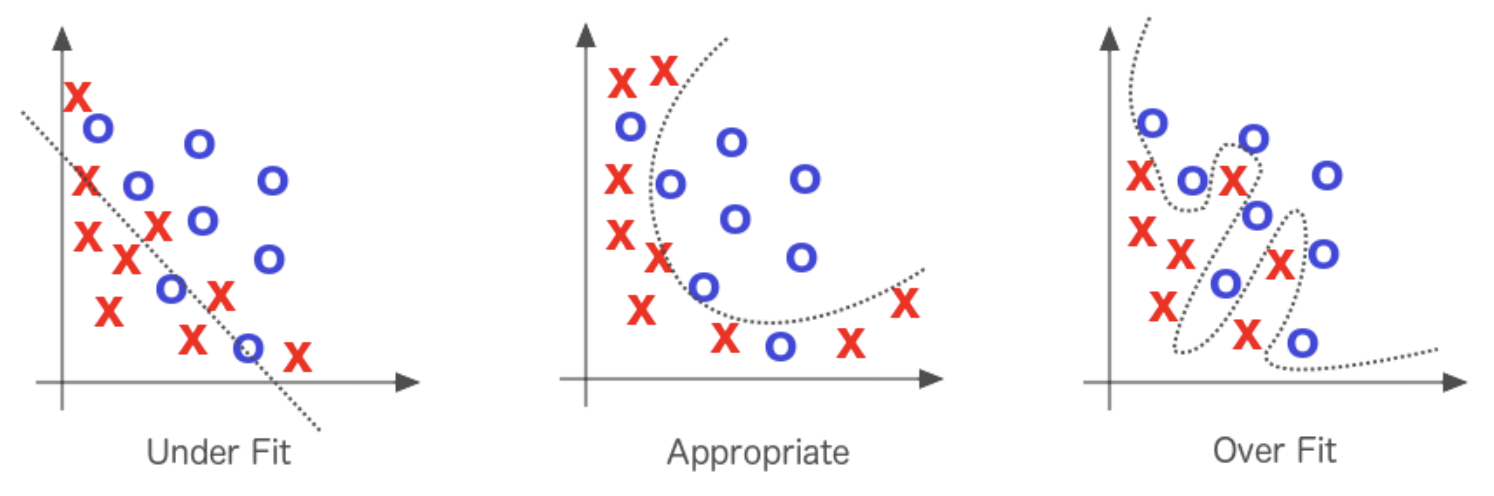
\includegraphics[width=10cm]{kapitel2/overundefit.png}
            \caption[Vergleich der Unteranpassung mit der Überanpassung]{Die Abbildung vergleicht die Überanpassung mit der Unteranpassung. Die einzelnen Punkte passen sich dem trainierten Model zu sehr an, der Verlust wird also so klein, dass das Modell nicht mehr zuverlässige Ergebnisse liefern kann. Dies ist darauf zurückzuführen, dass das Modell \enquote{zu viel} aus dem Trainingsdatensatz gelernt hat. Unteranpassung ist der Fall, wenn das Modell aus den Trainingsdaten \enquote{nicht genug gelernt} hat, was zu einer geringen Verallgemeinerung und unzuverlässigen Vorhersagen führt (Grafik entnommen aus \cite*[27]{Patterson2019}). }
            \label{Kap2:OverUnder}
        \end{figure}

        \section{Regularisierung}
        Die Regularisierung lässt die Auswirkungen von außer Kontrolle geratenen Parametern minimieren, indem verschiedene Methoden oder Strategien verwendet werden, um die Parametergröße im Laufe der Zeit zu minimieren. Der Hauptzweck der Regularisierung besteht darin, die Überanpassung zu kontrollieren \cite*[79]{Patterson2019}.

        Ein zentrales Problem beim maschinellen Lernen besteht darin, einen Algorithmus zu erstellen, der nicht nur bei den Trainingsdaten, sondern auch bei neuen Eingaben eine gute Leistung erbringt. Viele beim maschinellen Lernen verwendete Strategien sind explizit darauf ausgelegt, den Testfehler zu reduzieren, möglicherweise auf Kosten eines erhöhten Trainingsfehlers. Diese Strategien werden zusammen als Regularisierung bezeichnet. Tatsächlich war die Entwicklung effektiverer Regularisierungsstrategien eine der wichtigsten Forschungsanstrengungen auf diesem Gebiet. Regularisierung kann schließlich definiert werden als \enquote{jede Änderung, die wir an einem Lernalgorithmus vornehmen, um dessen Generalisierungsfehler, aber nicht seinen Trainingsfehler zu reduzieren} \cite*[228]{IanGoodfellowYoshuaBengio2016}.

        \subsection{Early Stopping}
        Wenn große Modelle trainiert werden, um eine bestimmte Aufgabe lösen, wird häufig festgestellt, dass der Trainingsfehler mit der Zeit stetig abnimmt, der Fehler des Validierungssatzes jedoch wieder zunimmt. Dies bedeutet, dass ein Modell mit einem besseren Validierungssatzfehler (und damit einem besseren Testsatzfehler) erhalten werden kann, indem zu dem Zeitpunkt mit dem niedrigsten Validierungssatzfehler zur Parametereinstellung zurückgekehrt wird. Jedes Mal, wenn sich der Fehler im Validierungssatz verbessert, wird eine Kopie der Modellparameter gespeichert. Wenn der Trainingsalgorithmus beendet wird, wird diese Parameter anstelle der neuesten Parameter zurückgegeben. Diese Strategie wird als \textbf{Early Stopping} \enquote{frühes Stoppen} bezeichnet. Es ist wahrscheinlich die am häufigsten verwendete Form der Regularisierung. Seine Popularität ist sowohl auf seine Wirksamkeit als auch auf seine Einfachheit zurückzuführen \cite*[246]{IanGoodfellowYoshuaBengio2016}.


        \subsection{Dropout}
        Eine weitere Strategie um Überanpassung zu vermeiden wird in \cite*{Srivastava2014} dargestellt. \textbf{Dropout} bietet eine rechnerisch kostengünstige, aber leistungsstarke Methode zur Regularisierung dar. Es ist das aufteilen des Netzwerkes in mehreren Teile. Es wird also ein Ensemble aus diesen kleinen Teilen (sub-networks) gebildet \cite*[258]{IanGoodfellowYoshuaBengio2016}.



        \begin{figure}[H]
            \centering
            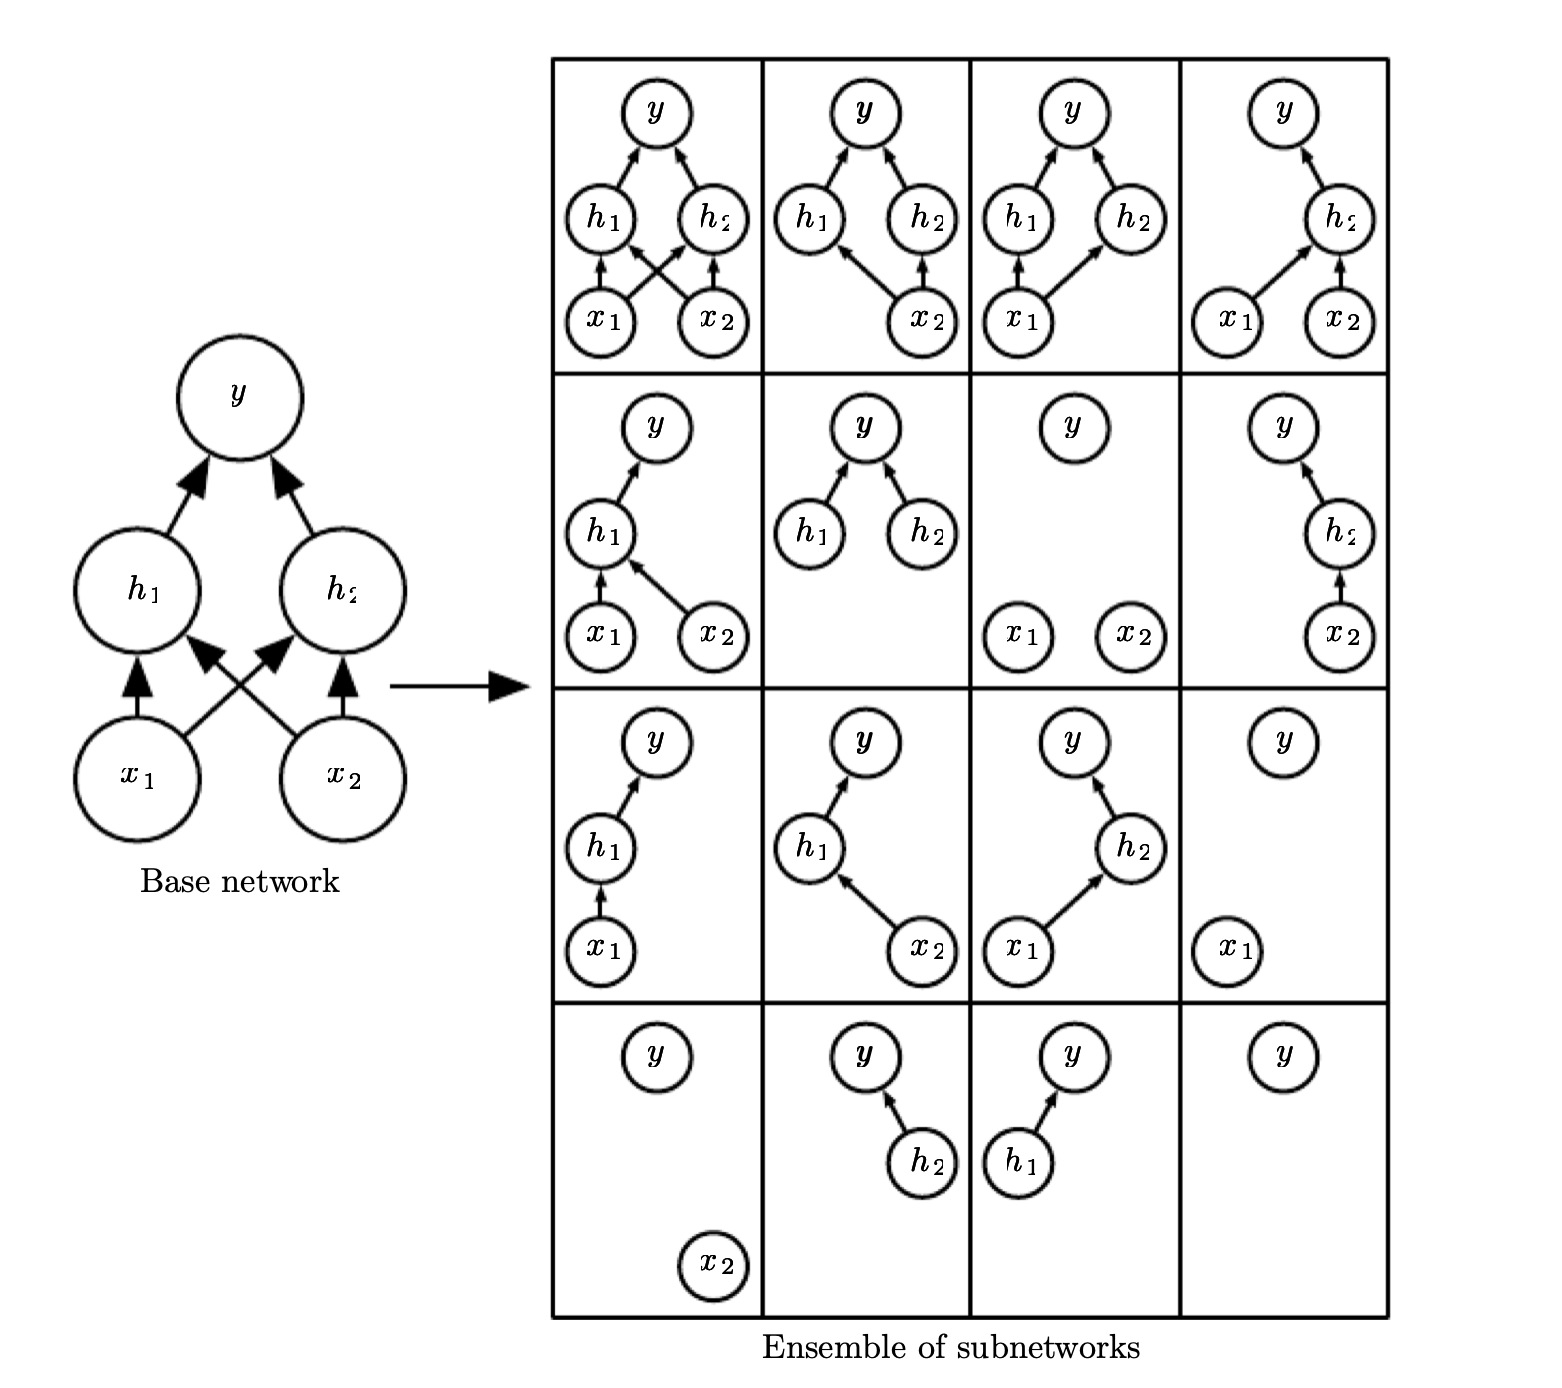
\includegraphics[width=10cm]{kapitel2/dropout.png}
            \caption[Basis-Netzwerks und Ensemble im Vergleich]{Dropout trainiert ein Ensemble. Ein Ensemble besteht aus allen Teilnetzwerken. Es wird durch das entfernen von Einheiten aufgebaut. Das Ensemble besteht aus 16 Teilmengen, aus den vier Einheiten des Basis-Netzwerks. Die 16 Subnetze werden durch das Löschen verschiedener Teilmengen von Einheiten aus dem ursprünglichen Netzwerk gebildet (entnommen aus \cite*[260]{IanGoodfellowYoshuaBengio2016}).}
            \label{Kap2:Dropout}
        \end{figure}

        \subsection{L1 und L2}
        Eine weitere Strategie der Regularisierung ist die Modifikation der L1 und L2 Gewichte. Beim Deep Learning wird die Größe von Vektoren mit einer Funktion, die als \enquote{Norm} bezeichnet wird \cite*[39]{IanGoodfellowYoshuaBengio2016} gemessen. Formal ist diese Norm $L^p$ gegeben als:

        \begin{equation} \label{FormelNorm2}
            \Vert x\Vert \ =\ \left(\sum _{i}\bigr| x_{i}\bigr|^{p}\right)^{\frac{1}{p}}.
        \end{equation}

        Normen, einschließlich der $L^p$-Norm, sind Funktionen, die Vektoren auf nicht negative Werte abbilden. Auf einer intuitiven Ebene misst die Norm eines Vektors $x$ den Abstand vom Ursprung zum Punkt $x$. Die $L^2$-Norm mit $p = 2$ als euklidische Norm bekannt. Es ist der euklidische Abstand vom Ursprung zum Punkt $x$. Die $L^2$-Norm wird beim maschinellen Lernen häufig verwendet, sie wird einfach als $\Vert x\Vert$ bezeichnet, wobei der Index 2 weggelassen wird \cite*[39]{IanGoodfellowYoshuaBengio2016}.

        Wenn zwischen Elementen zu unterscheiden ist, die genau Null sind und Elementen die klein, aber ungleich Null sind, wird die $L^1$-Norm angewendet. Die $L^1$-Norm kann vereinfacht werden als \cite*[40]{IanGoodfellowYoshuaBengio2016}:

        \begin{equation} \label{FormelNorm1}
            \Vert x\Vert 1\ =\ \sum _{i}\bigr| x_{i}\bigr|.
        \end{equation}


        \section{Verlustfunktion und Kreuzentropie}
        \subsection{Verlustfunktionen}
        Innerhalb eines neuronalen Netzwerks wandelt eine \textbf{Verlustfunktion} oder \textbf{Kostenfunktion} alle möglichen Fehler, in eine Zahl um, die den Gesamtfehler des Netzwerks darstellt. Im Wesentlichen ist es ein Maß dafür, wie falsch ein Netzwerk liegt.

        Das Neuron lernt dadurch, indem es Gewichte und Bias mit einer Rate ändert, die durch die partiellen Ableitungen der Kostenfunktion $\partial$$C$/$\partial$$w$ und $\partial$$C$/$\partial$$b$ bestimmt wird. Zu sagen, dass das \enquote{Lernen langsam ist}, ist also dasselbe wie zu sagen, dass diese partiellen Ableitungen klein sind \cite*[61]{Nielsen2015}. Gegeben sei die quadratische Verlustfunktion:

        \begin{equation} \label{Formel2_5}
            C=\frac{( y-a)^{2}}{2},
        \end{equation}

        dabei ist $a$ die Ausgabe des Neurons, wenn die Trainingseingabe $x = 1$ ist, und $y = 0$ die entsprechende gewünschte Ausgabe. Um dies in Bezug auf Gewicht und Bias expliziter zu schreiben, sei daran erinnert, dass $a = \sigma(z)$ ist, wobei $z = wx + b$ ist. Es ergeben sich durch die Anwendung der Kettenregel folgende Gleichungen:

        \begin{equation} \label{Formel2_6}
            \frac{\partial C}{\partial w} =( a-y) \sigma '( z) x=a\sigma '( z)
        \end{equation}

        \begin{equation} \label{Formel2_7}
            \frac{\partial C}{\partial b} =( a-y) \sigma '( z) =a\sigma '( z).
        \end{equation}

        Aus der Abbildung~\ref{Kap2:Sigmoid_plot} ist die Kurve der Sigmoidfunktion zu sehen. Die Kurve wird sehr flach, wenn der Ausgang des Neurons nahe bei 1 liegt, und daher wird $\sigma'(z)$ sehr klein. Die Gleichungen~\ref{Formel2_6} und ~\ref{Formel2_7} sagen dann aus, dass $\partial$$C$/$\partial$$w$  und  $\partial$$C$/$\partial$$b$ sehr klein werden. Dies ist der Grund warum das lernen langsamer wird.

    \subsection{Kreuzentropie}
    Nach \cite*[62]{Nielsen2015} kann die Lernverlangsamung gelöst werden, indem die quadratische Verlustfunktion durch eine andere Verlustfunktion ersetzt wird. Diese Funktion wird als als \textbf{Kreuzentropie} bezeichnet. Die Abbildung~\ref{Kap2:Entropie} zeigt die Kreuzentropie mit mehreren Eingabevariablen und entsprechenden Gewichten und dem Bias. Die Ausgabe des Neurons ist $a = \sigma(z)$, wobei $z =  \sum _{j} w_{j} b_{j} + b$ ist, die gewichtete Summe des Inputs. Die Kreuzentropiekostenfunktion für dieses Neuron wird definiert durch:

    \begin{equation} \label{Formel2_8}
        C=\ -\frac{1}{n}\sum _{x}[ y\ ln\ a\ +\ ( 1-y) \ ln( 1-a)]
    \end{equation}

    wobei $n$ die Gesamtzahl der Trainingselemente darstellt. Die Summe gibt die entsprechende gewünschte Ausgabe $x$ und $y$ über alle Trainingseingaben an. Zusammenfassend ist die Kreuzentropie positiv und tendiert gegen Null, wenn das Neuron
    \enquote{besser} wird in der Berechnung der gewünschten Ausgabe $y$ für alle Trainingseingaben $x$ ist.  Die entropieübergreifende Kostenfunktion hat jedoch den Vorteil, dass sie im Gegensatz zu den quadratischen Kosten das Problem der Verlangsamung des Lernens vermeidet. Um dies zu sehen, wird die partielle Ableitung der Kreuzentropiekosten in Bezug auf die Gewichte berechnet \cite*[63]{Nielsen2015}.

    \begin{gather} \label{Formel2_9}
        \frac{\partial C}{\partial w_{j}} =-\frac{1}{n}\sum _{x}\left(\frac{y}{\sigma ( z)} -\frac{1-y}{1-\sigma ( z)}\right)\frac{\partial \sigma }{\partial w_{j}} = \notag\\
        -\frac{1}{n}\sum _{x}\left(\frac{y}{\sigma ( z)} -\frac{1-y}{1-\sigma ( z)}\right) \sigma '( z) x_{j}
    \end{gather}

    \begin{equation} \label{Formel2_10}
        \frac{\partial C}{\partial w_{j}} \ =\ \frac{1}{n}\sum _{x}\frac{\sigma '( z) x_{j}}{\sigma ( z)( 1-\sigma ( z))}( \sigma ( z) -y)
    \end{equation}

    \begin{equation} \label{Formel2_11}
        \frac{\partial C}{\partial w_{j}} \ =\ \frac{1}{n}\sum _{x} x_{j}( \sigma ( z) -y)
    \end{equation}


    Die Geschwindigkeit, mit der das Gewicht $w$ lernt, wird durch $\sigma(z) - y$ gesteuert, also durch den Fehler in der Ausgabe. Je größer dieser Fehler wird, desto schneller lernt das Neuron. Dies ist ein gewünschtes Verhalten. Insbesondere wird die Lernverlangsamung vermieden, die durch den Term $\sigma'(z)$ in der analogen Gleichung für die quadratischen Kostenfunktion~\ref{Formel2_6} verursacht wird. Wenn die Kreuzentropie verwendet wird, wird der Term $\sigma'(z)$ aufgehoben und somit ist es egal, ob es klein ist. Diese Aufhebung ist das Besondere, welches durch die Kreuzentropie-Kostenfunktion gewährleistet wird \cite[63-64]{Nielsen2015}.

    \begin{figure}[H]
        \centering
        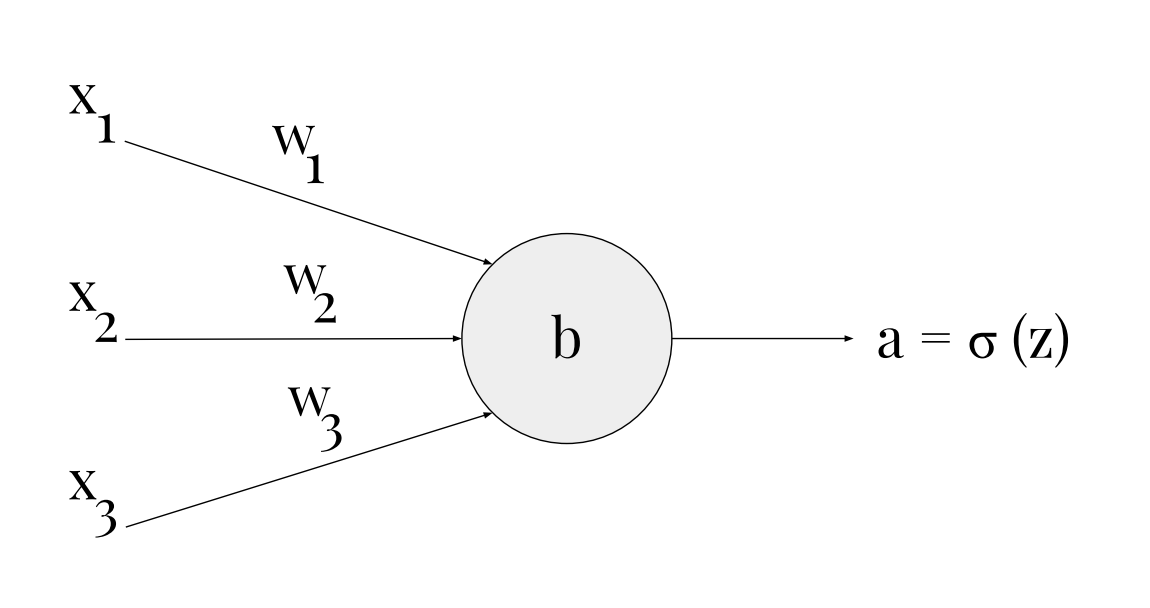
\includegraphics[width=8cm]{kapitel2/entropie.png}
        \caption[Darstellung der Kreuzentropie am beispiel eines Neurons]{Das Neuron wird mit 3 Eingabewerten $(x_1, x_2, x_3)$ den dazugehörigen Gewichten $(W_1, W_2, W_3)$ trainiert. Der Bias ist durch $b$ angegeben und die Ausgabe mit $a = \sigma(z)$ (in Anlehnung an \cite*{Nielsen2015})}
        \label{Kap2:Entropie}
    \end{figure}

    \section{Convolutional Neural Network}

    ConvNets/CNNs oder \textbf{Convolutional Neural Networks} dienen zur Verarbeitung von Daten in Form mehrerer Arrays, beispielsweise eines Farbbilds aus drei 2D-Arrays mit Pixelintensitäten in den drei Farbkanälen. Viele Datenmodalitäten liegen in Form mehrerer Arrays vor: 1D für Signale und Sequenzen, einschließlich Sprache; 2D für Bilder oder Audiospektrogramme; und 3D für Video- oder Volumenbilder. Hinter ConvNets stehen vier Schlüsselideen, die die Eigenschaften natürlicher Signale nutzen: lokale Verbindungen, gemeinsame Gewichte, Pooling und die Verwendung vieler Schichten \cite*{Lecun2015}.


    CNNs arbeiten mit gitterstrukturierten Eingaben, die in lokalen Regionen des Netzes starke räumliche Abhängigkeiten aufweisen. Das offensichtlichste Beispiel für gitterstrukturierte Daten ist ein zweidimensionales Bild. Diese Art von Daten weisen räumliche Abhängigkeiten auf, da benachbarte räumliche Orte in einem Bild häufig ähnliche Farbwerte der einzelnen Pixel aufweisen. Eine zusätzliche Dimension erfasst die verschiedenen Farben, wodurch ein dreidimensionales Eingabevolumen entsteht. Andere Formen von sequentiellen Daten wie Text, Zeitreihen und Sequenzen können ebenfalls als Sonderfälle von Daten mit Gitterstruktur mit verschiedenen Arten von Beziehungen zwischen benachbarten Elementen betrachtet werden. Die überwiegende Mehrheit der Anwendungen von CNNs konzentriert sich auf Bilddaten, obwohl man diese Netze auch für alle Arten von zeitlichen, räumlichen und raumzeitlichen Daten verwenden kann. Ein wichtiges definierendes Merkmal von CNNs ist eine Operation, die als Faltung (convolution) bezeichnet wird. \cite*[315-316]{Aggarwal2018}.




    \subsection{Architektur}
    In CNNs sind mehrere Schichten miteinander verbunden und jeder Schicht hat eine Gitterstruktur. Die Bezihungen zwischen den Schichten werden von einer Schicht zur nächsten vererbt, da jeder Merkmalswert auf einem kleinen lokalen Bereich aus der vorherigen Schicht basiert. Es ist wichtig, diese räumlichen Beziehungen zwischen den Gitterzellen aufrechtzuerhalten, da die Faltungsoperation und die Transformation zur nächsten Schicht von diesen Beziehungen abhängen. Jede Schicht im Faltungsnetzwerk ist eine dreidimensionale Gitterstruktur mit einer Höhe, Breite und Tiefe. Die Tiefe einer Schicht in einem Faltungsnetzwerk ist nicht die Tiefe des Netzwerks selbst. Das Wort \enquote{Tiefe} bezieht sich auf die Anzahl der Kanäle in jeder Ebene, z. B. die Anzahl der Primärfarbkanäle (z. B. Blau, Grün und Rot) im Eingabebild \cite*[318]{Aggarwal2018}.

    Die Architektur eines typischen ConvNets ist in mehrere Phasen unterteilt. Die ersten Stufen bestehen aus zwei Arten von Schichten: Faltungsschichten und Poolschichten. Einheiten in einer Faltungsebene sind in \textbf{Feature-Maps} organisiert, in denen jede Einheit über eine Reihe von Gewichten, die als Filterbank bezeichnet werden, mit lokalen Patches in den Feature-Maps der vorherigen Ebene verbunden ist. Das Ergebnis dieser lokal gewichteten Summe wird dann durch eine Nichtlinearität wie \zb eine ReLU geleitet. Alle Einheiten in einer Feature-Map verwenden dieselbe Filterbank\cite*{Lecun2015}.


    \begin{figure}[H]
        \centering
        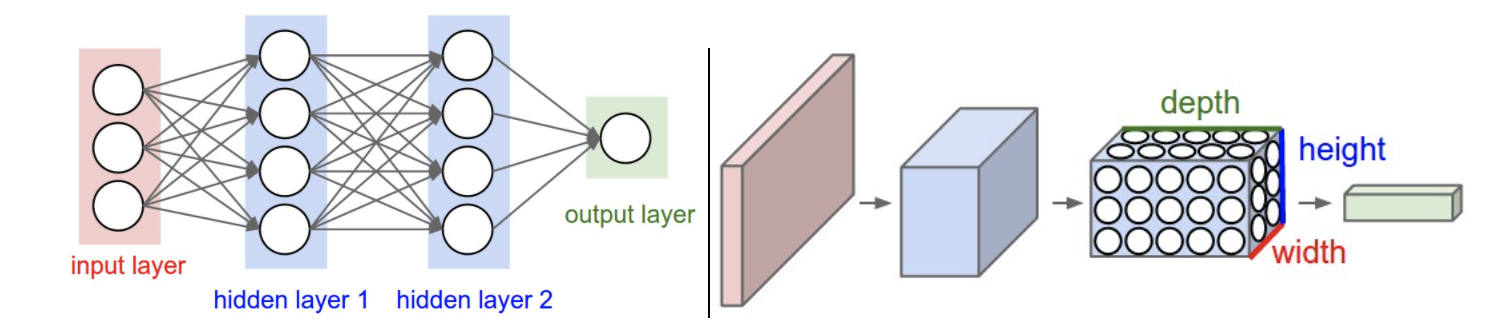
\includegraphics[width=13cm]{kapitel2/conv.png}
        \caption[Vergleich eines NN mit einem CNN]{Links: Ein reguläres 3-Schicht-Neuronales Netz. Rechts: Ein ConvNet ordnet seine Neuronen in drei Dimensionen (Breite, Höhe, Tiefe) an, wie in einer der Ebenen dargestellt. Jede Schicht eines ConvNet wandelt das 3D-Eingangsvolumen in ein 3D-Ausgangsvolumen von Neuronenaktivierungen um. In diesem Beispiel enthält die rote Eingabeebene das Bild, sodass seine Breite und Höhe den Abmessungen des Bildes entsprechen. Die \enquote{Tiefe} sind die 3 Farbkanäle (rot, grün, blau) aus \cite*{StanfordUniversityCoursecs231n2018a}.}
        \label{Kap2:Conv}
    \end{figure}


    \subsection{Convolutional Layer}

    Die Parameter der  \textbf{Convolutional Layer} oder \textbf{Faltungsschicht} bestehen aus einer Reihe von lernbaren Filtern. Jedes dieser Filter ist räumlich klein (Breite und Höhe), erstreckt sich jedoch über die gesamte Tiefe des Eingangsvolumens. Beispielsweise könnte ein typischer Filter auf einer ersten Schicht eines ConvNet die Größe \textit{5 × 5 × 3} haben (d. H. 5 Pixel Breite und Höhe und 3, weil Bilder die Tiefe 3 haben, also die Farbkanäle). Während des Vorwärtsdurchlaufs wird jedes der Filter über die Breite und Höhe des Eingangsvolumens \textit{gefaltet} und es werden die Punktprodukte zwischen den Einträgen des Filters und dem Eingang an einer beliebigen Position berechnet. Wenn der Filter über die Breite und Höhe des Eingangsvolumens gefaltet wird, wird eine zweidimensionale \textit{Aktivierungskarte} (feature map) erstellt, die die Antworten dieses Filters an jeder räumlichen Position angibt. Intuitiv lernt das Netzwerk Filter, die aktiviert werden, wenn sie eine Art visuelles Merkmal sehen, z. B. eine Kante mit einer bestimmten Ausrichtung oder einen Farbfleck auf der ersten Ebene oder schließlich radähnliche Muster auf höheren Ebenen des Netzwerks. Es entstehen somit ein ganzer Satz von Filtern in jeder Faltungsschicht (z. B. 12 Filter), und jeder von ihnen erzeugt eine separate zweidimensionale Aktivierungskarte. Diese Karten werden entlang der Tiefendimension gestapelt und das Ausgabevolumen erzeugt \cite*{StanfordUniversityCoursecs231n2018a}.

    \begin{figure}[H]
        \centering
        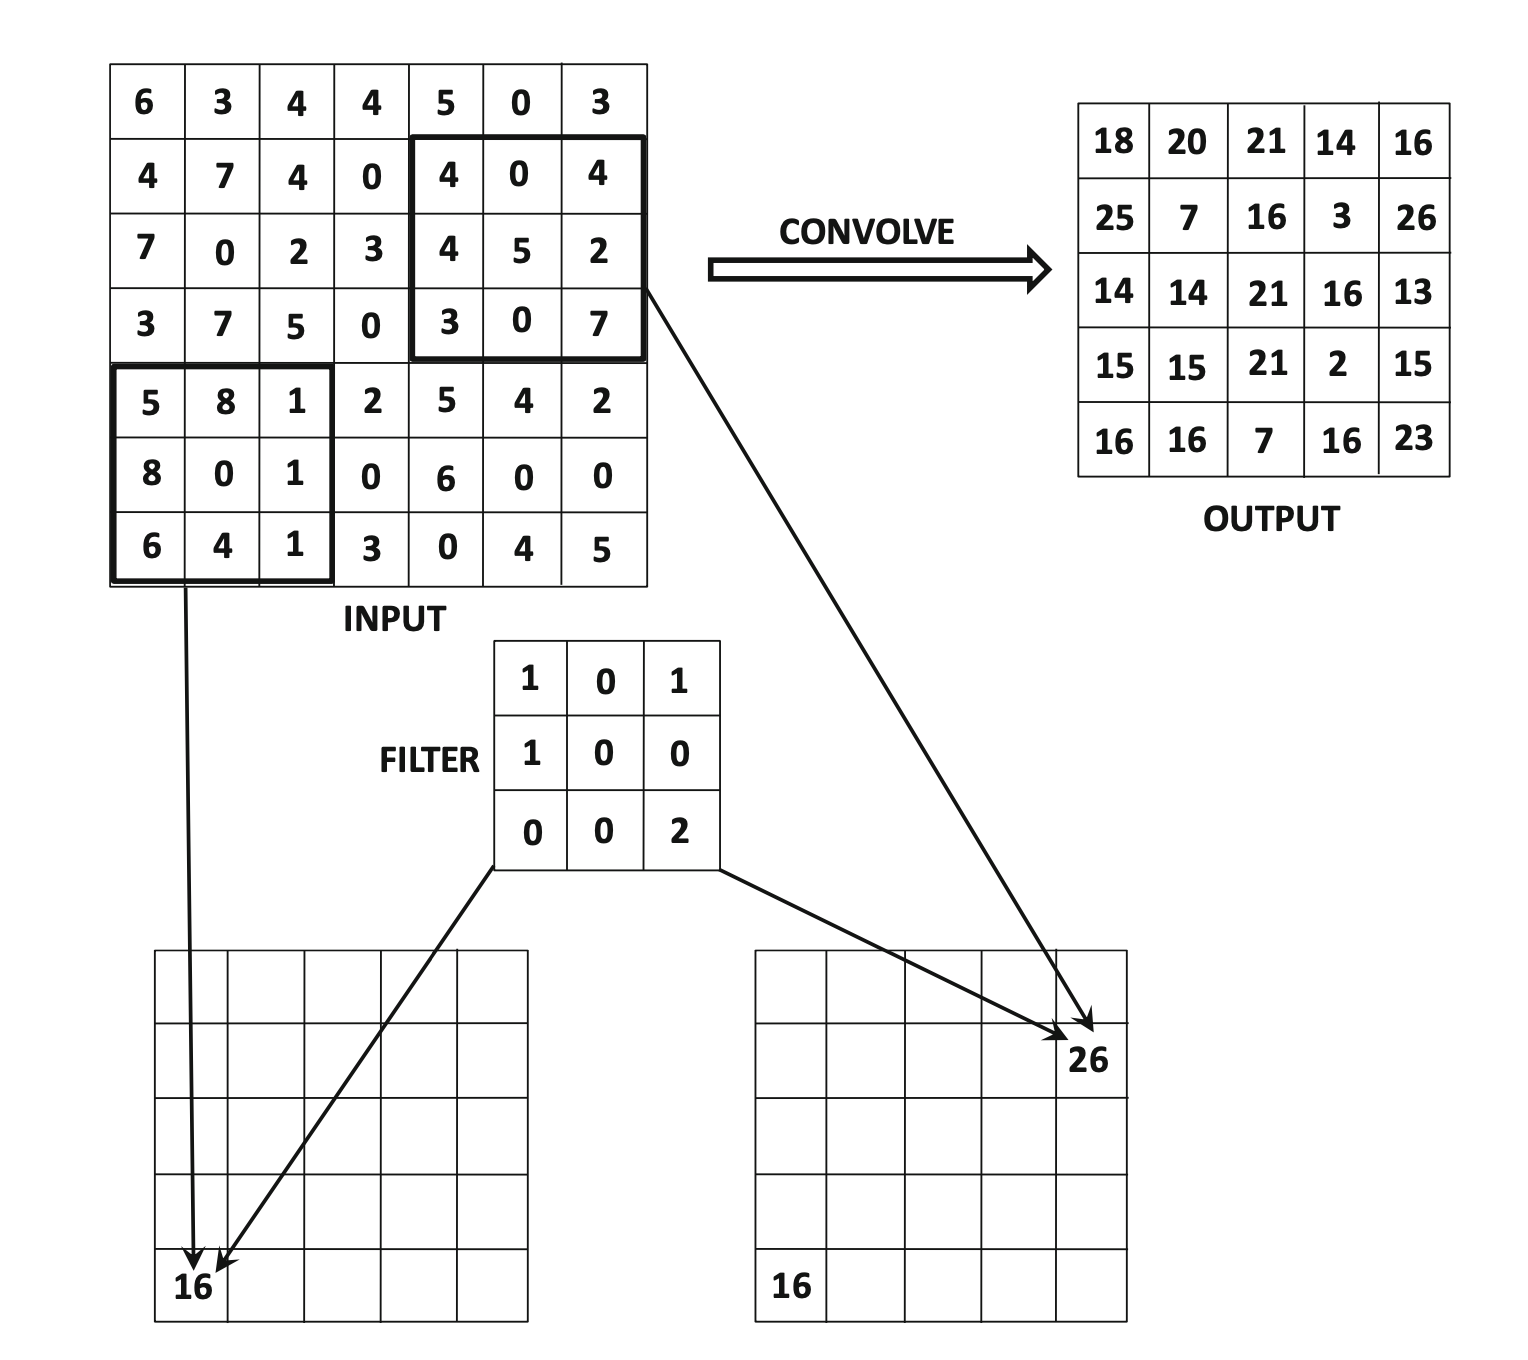
\includegraphics[width=10cm]{kapitel2/conv_layers.png}
        \caption[Die Faltung in einem CNN]{Die Faltungsoperation geschieht durch eine Punktprodukt Operation des Filters, was über alle räumlichen Positionen wiederholt wird aus \cite*[321]{Aggarwal2018}.}
        \label{Kap2:Conv}
    \end{figure}

    \subsubsection{Padding}
    Die Faltungsoperation verringert die Größe der $(q + 1)$-ten Schicht im Vergleich zur Größe der $q$-ten Schicht. Diese Art der Größenreduzierung ist im Allgemeinen nicht wünschenswert, da sie dazu neigt, einige Informationen entlang der Bildränder zu verlieren. Dieses Problem kann durch \textbf{Auffüllen} (padding) gelöst werden. Beim Auffüllen werden neue Werte rund um die Ränder der Feature-Map hinzugefügt. Der Wert jedes dieser aufgefüllten Feature-Werte wird auf 0 gesetzt, unabhängig davon, ob die Eingabe oder die ausgeblendeten Ebenen aufgefüllt werden. Diese Bereiche tragen nicht zum endgültigen Punktprodukt bei, da ihre Werte auf 0 gesetzt sind. Ein Teil des Filters aus den Rändern der Schicht wird \enquote{herausragt} und dann durch das Durchführen des Punktprodukts nur über den Teil der Ebene, in dem die Werte definiert sind ersetzt \cite*[323]{Aggarwal2018}.


\subsection{Pooling Layer}
Es ist üblich, regelmäßig eine \textbf{Pooling Ebene} zwischen aufeinanderfolgenden Faltungsebenen in eine ConvNet-Architektur einzufügen. Die Funktion dieser Ebenene besteht darin, die räumliche Größe der Darstellung schrittweise zu verringern, um die Anzahl der Parameter und die Berechnung im Netzwerk zu verringern und damit auch die Überanpassung zu steuern. Die Pooling-Ebene arbeitet unabhängig mit jedem Tiefenabschnitt der Eingabe und ändert die Größe räumlich mithilfe der MAX-Operation. Die gebräuchlichste Form ist eine Pooling-Ebene mit Filtern der Größe \textit{2x2}, die mit einem\textbf{ Schritt} (Stride) von 2 Downsamples pro Tiefenscheibe in der Eingabe um 2 entlang der Breite und Höhe angewendet werden, wobei 75\% der Aktivierungen verworfen werden. Jede MAX-Operation würde in diesem Fall maximal 4 Zahlen annehmen. Der \textit{Volumen} bleibt unverändert \cite*{StanfordUniversityCoursecs231n2018a}.

\begin{figure}[H]
    \centering
    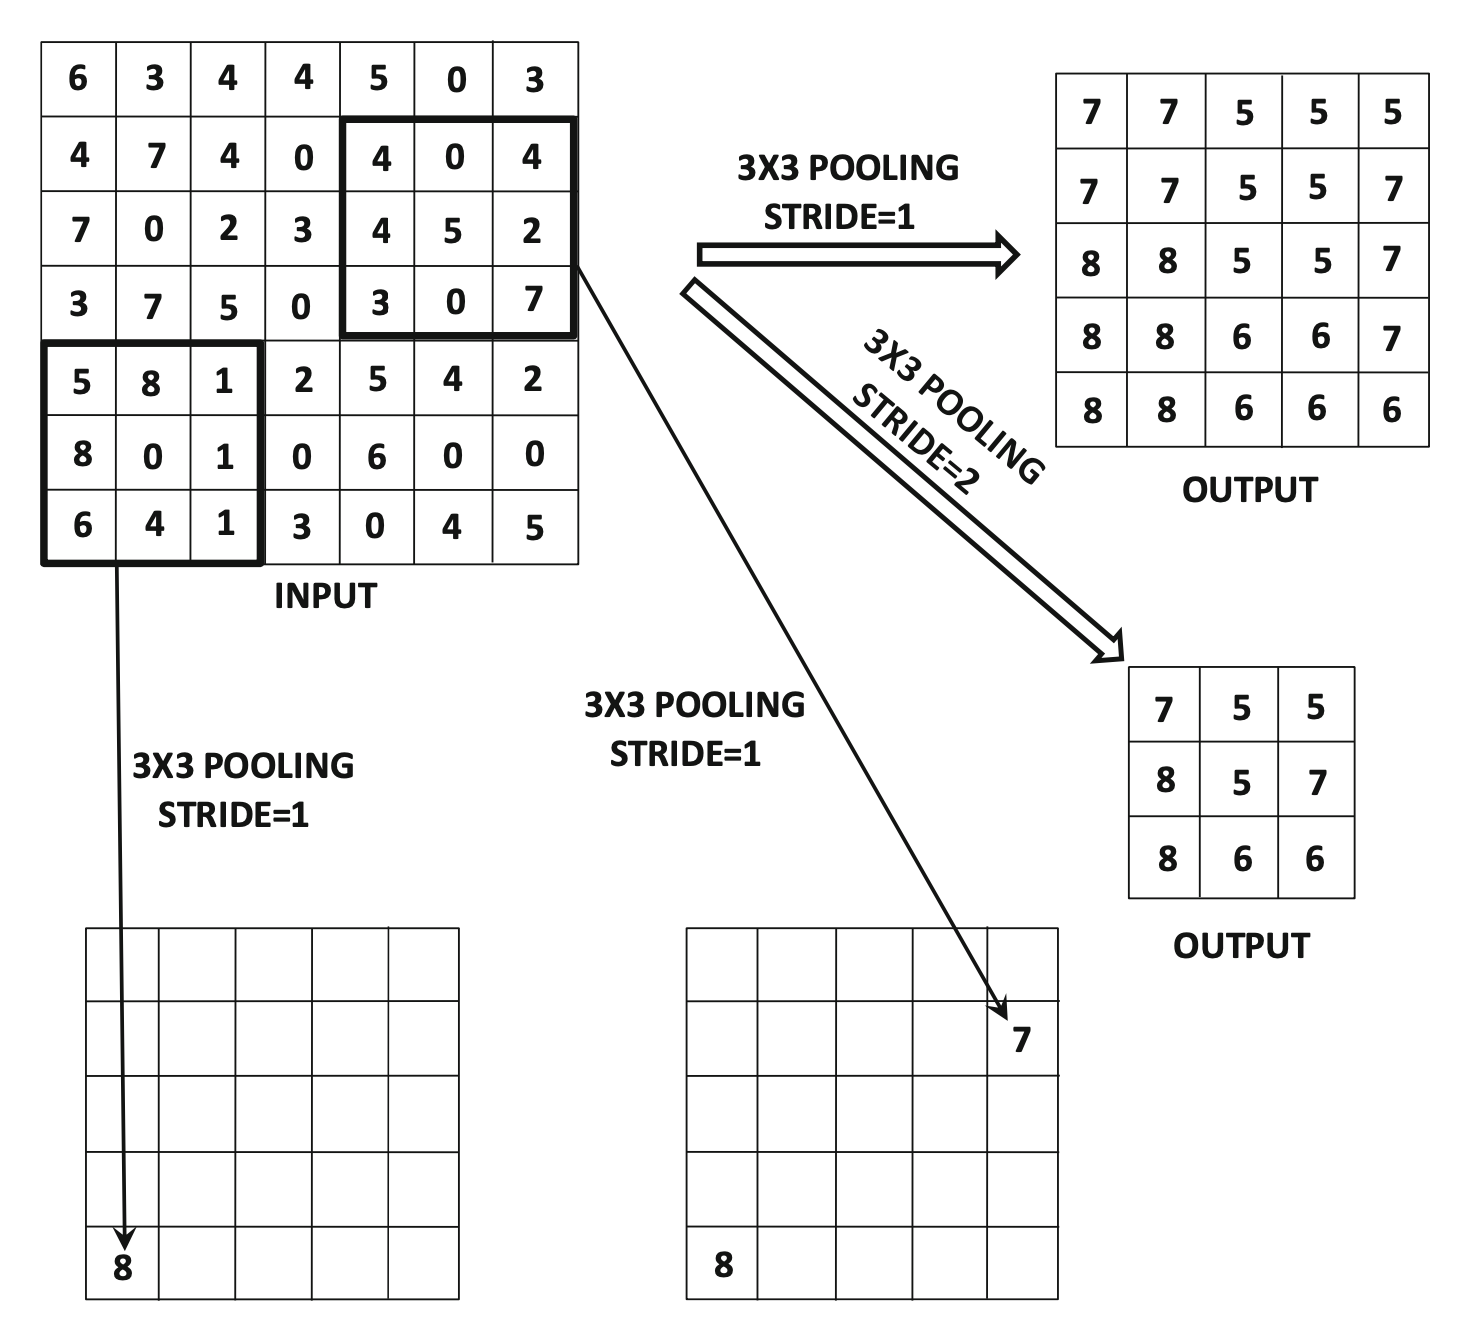
\includegraphics[width=9cm]{kapitel2/maxpooling.png}
    \caption[Max-Pooling]{Ein Beispiel für ein Max-Pooling einer Aktivierungskarte der Größe 7 × 7 mit Stride von 1 und 2. Ein Stride von 1 erzeugt eine 5 × 5-Aktivierungskarte mit stark wiederholten Elementen aufgrund der Maximierung in überlappenden Regionen. Ein Stride von 2 erzeugt eine 3 × 3-Aktivierungskarte mit weniger Überlappung \cite*[326]{Aggarwal2018}.}
    \label{Kap2:Pooling}
\end{figure}


\subsection{Vollständig verbundene Ebenen}
Am Ende wird die sogenannte \textbf{vollständig verbundene Ebenen} des Netzwerkes verwendet, um Klassenwerte zu berechnen, die als Ausgabe des Netzwerks dienen sollen. In einem traditionellen vorwärtsgerichteten Neuronalen Netzwerk wird jedes Eingangsneuron mit jedem Ausgangsneuron in der nächsten Schicht verbunden. Dies wird auch als vollständig verbundene Schicht bezeichnet. Der einzige Unterschied zwischen der vollständig verbundene Ebene und Faltungsschichten besteht darin, dass die Neuronen in der Faltungsschicht nur mit einer lokalen Region der Eingabe verbunden ist. Die Neuronen in beiden Schichten berechnen jedoch immer noch Punktprodukte, sodass ihre funktionale Form identisch ist. Zwischen beiden Schichten ist eine Konvertierung möglich \cite*{StanfordUniversityCoursecs231n2018a}.



%   \section{Backpropagation}
%   Wenn vorwärts gerichtetes neuronales Netzwerk (\enquote{feedforward neural network}) verwenden, um eine Eingabe $x$ zu anzunehmen und eine Ausgabe $y$ zu erzeugen, fließen die Informationen durch das Netzwerk vorwärts. Die Eingaben $x$ liefern die initialen Informationen, die sich dann bis zu den verborgenen Einheiten (\enquote{hidden layers}) auf jeder Schicht ausbreiten und schließlich die Ausgabe erzeugen. Dies wird als (\enquote{forward propagation}) bezeichnet. Während des Trainings kann die also die Ausbereitung nach vorne fortgesetzt werden. Der Back-Propagation-Algorithmus \cite*{Rumelhart1986}, oft einfach Backprop genannt, ermöglicht es den Informationen, rückwärts durch das Netzwerk zu fließen \cite[204]{IanGoodfellowYoshuaBengio2016}.

%   Das Herzstück der Backpropagation ist ein Ausdruck aus der partiellen Ableitung, $\partial C$ / $\partial w$ wo die Kostenfunktion $C$ in Bezug auf ein beliebiges Gewicht $w$ (oder einen Bias $b$) im Netzwerk ist. Der Ausdruck sagt uns, wie schnell sich \enquote{die Kosten ändern}, wenn wir die Gewichte und den Bias ändern. Backpropagation gibt uns detaillierte Einblicke, wie das Ändern der Gewichte und des Bias das Gesamtverhalten des Netzwerks verändert \cite*[39]{Nielsen2015}.

% Das Training eines neuronalen Netzwerks bedeutet im Grunde, alle \enquote{Gewichte} zu kalibrieren, indem zwei Schritte wiederholt werden: Forward Pagation und Backpropagation. Beim Forward Pagation wenden wir eine Reihe von Gewichten auf die Eingabedaten an und berechnen eine Ausgabe. Für die erste Forward Pagation werden die Gewichte zufällig ausgewählt. Beim Backpropagation messen wir die Fehlerquote der Ausgabe und passen die Gewichte entsprechend an, um den Fehler zu verringern. Neuronale Netze wiederholen sowohl die Forward Pagation als auch die Backpropagation, bis die Gewichte kalibriert sind, um eine Ausgabe genau vorherzusagen \cite{Miller}.

% Durch Forward Pagation machen neuronale Netze also Vorhersagen. Eingabedaten werden Schicht für Schicht durch das Netzwerk an die letzte Schicht weitergeleitet, die eine Vorhersage ausgibt. Die Ziele der Backpropagation sind das Anpassen jedes Gewicht im Netzwerk proportional dazu, wie viel es zum Gesamtfehler beiträgt. Wenn wir den Fehler jedes Gewichts iterativ reduzieren, haben wir schließlich eine Reihe von Gewichten, die gute Vorhersagen liefern.


% \section{Formelsatz}

% Eine Formel gefällig? Mitten im Text $a_2 = \sqrt{x^3}$ oder als eigener Absatz (siehe Formel~\ref{Formel}):




% Das Aufkommen von Online-Nachrichtenagenturen und die Explosion der Anzahl der Benutzer, die Nachrichten mit diesem Medium konsumieren, haben dazu geführt, dass mehrere Webseiten miteinander konkurrieren, um die Aufmerksamkeit der Benutzer zu erregen. Dies hat dazu geführt, dass Verkaufsstellen kreative Wege geschaffen haben, um Leser auf ihre Website zu locken. Eine der am häufigsten verwendeten Techniken ist die Verwendung von Clickbait-Überschriften. Diese Überschriften wurden speziell dafür entwickelt, um das Interesse des Lesers an dem zu wecken, was versprochen wird. Wenn auf den Artikel geklickt wird jedoch, liefert dieser Artikel normalerweise nicht den Inhalt, den der Leser Ursprüngich gesucht hat. In den Abbildungen \ref{Kap2:ClickBait} und \ref{Kap2:News}\footnote{Entnommen aus: https://github.com/MichaelGoodale/Clickbait-Classifier} wird der Unterschied zwischen Clickbaits und \enquote{normalen} Nachrichten aufgezeigt.

% \begin{figure}
%   \centering
%   \includegraphics[width=12cm]{kapitel2/clickbait.png}
%   \caption[Beispiel von Clickbait]{Beispiel von Clickbait}
%   \label{Kap2:ClickBait}
% \end{figure}


% \begin{figure}[ht]
%   \centering
%   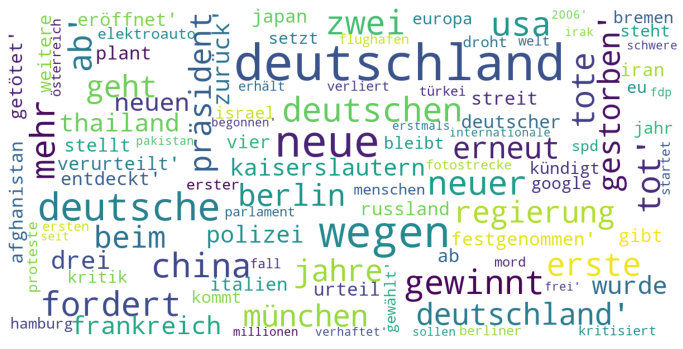
\includegraphics[width=12cm]{kapitel2/news.png}
%   \caption[Beispiel von \enquote{normalen} Nachrichten]{Beispiel von \enquote{normalen} Nachrichten}
%   \label{Kap2:News}
% \end{figure}


% \section{Lösungsansatz}
% Textklassifizierung ist eine gängige Art, wie man \enquote{gute} von \enquote{bösen} Texten unterscheiden kann. Es ist allerdingt nicht praktisch ein großes Sprachmodell wie GPT-3 Browserkompatible zu machen. Erstens ist es völlig \enquote{overkill} für ein solches Problem ein Sprachmodell zu benutzen und zweitens passen diese großen Modelle nicht in den Browser, da die Ladezeit nicht praktisch ist.

% Mit dieser Arbeit möchte ich ein Modell erstellen, um Clickbait Überschriften zu erkennen. Es wäre Hilfreich, wenn es ein Dienst gibt, welches eine Überschrift liest und dem Benutzer vorhersagt, ob es sich um Clickbait handelt oder nicht. So kann der Nutzer seine Zeit sparen und muss nicht auf die Seite gehen. Das Hauptprodukt ist dabei dieser Dienst, welches ganz einfach in jede HTML-Seite importiert werden kann. Dieser Dienst muss klein und schnell und gute dabei möglichst Ergebnisse liefern.

% \section{Aufbau der Arbeit}


% Im Abschnitt 2.6 Grobgliederung befindet sich eine mögliche Gliederung für diese Arbeit, auf die ich verweisen möchte. Zunächst wird in den Kapiteln 2 und 3 eine theoretische Grundlage geschaffen. Diese Kapitel beschäftigen sich mit Deep Learning und den mathematisch/statistschischen Erklärungen. Kapitel 3 orientiert sich eher mit NLP und insbesondere mit Worteinbettungen und wie moderne Computer die natürliche Sprache verstehen. Kapitel 4 soll den aktuellen Forschungsstand mit meiner Arbeit vergleichen. Es sollen verwandte Lösungsansätze kategorisch analysiert werden.

% Um mit dem eigentlichen Kern anzufangen, benötigt diese Arbeit an Daten. In Kapitel 5 wird gezeigt wie mittelt Webscraping. Dieser Datensatz wird händisch gelabelt und besteht aus einem Titel und einer Klasse. Die erste erste hälfte des Datensatzes wird aus Wikinews\footnote{https://de.wikinews.org/wiki/Hauptseite} geladen. Wikinews hat einen API-Zugang wodurch Nachrichten, welche nicht Clickbait sind in den Datensatz gebracht werden können. Ich habe dafür bereits mehr als 10.000 Nachrichten-Titel in eine Datenbank geladen. Die zweite hälfte des Datensatzes wird mittels Webseiten mit Scrapy\footnote{ https://scrapy.org/} gescraped. Die ersten 1.000 Titel sind bereits in die Datenbank\footnote{https://github.com/youurt/klickkoeder/blob/main/klickscraper/klickscraper.db} geladen worden.

% Nachdem ausreichend Daten geladen werden, ist geplant diese Daten zu laben. Damit später keine Verzerrungen bei den Daten entstehen, plane ich noch eine weitere Person zum Unterstützen beim Labeln mit in die Arbeit zu nehmen. Dieses wird mit dem Betreuer der Arbeit noch abgeklärt werden müssen. Der restliche Teil dieses Kapitels beschäftigt sich mit der Analyse der Daten um bestimmte Muster zu erkennen und die Daten in ein passendes Format zu bringen.

% Ich werde ein Modell in TensorFlow.js entwickeln. Dieses Modell soll möglichst klein sein und schnell sein. Um mit TensorFlow.js arbeiten zu können muss der Text in Vektoren umgewandelt werden.

% Mit einem Versuchsaufbau soll das Modell getestet und analysiert werden. Schließlich soll das Modell in die Browser-Umgebung gebracht und mittels eines minimalistischen React Frontends angeboten werden.

% \begin{figure}[ht]
%   \centering
%   \includegraphics[width=12cm]{kapitel2/beispiel.png}
%   \caption[Beispiel einer Systemarchitektur]{Beispiel einer Systemarchitektur entnommen aus \cite{cho2019shop}. Der Client bekommt beim laden der Seite, neben dem HTML, CSS und dem JavaScript, welches für das Frontend nötig ist, ein weiteres Script, welches die TensorFlow.js API bereitstellt. Die Berechnung findet im Browser, beim Client statt, wo auch das Modell sich befindet.}
%   \label{Kap2:SystemArchitektur}
% \end{figure}

% \section{Wissenschaftlicher Beitrag}
% \begin{itemize}
%   \item Den Stand der Technik in Bezug auf Deep Learning und Worteinbettungen zeigen
%   \item Erstellung und labeln eines Datensatzes für deutsche Clickbaits
%   \item Implementierung eines NLP-Problemes im Browser ohne zusätzliche Software oder Plugins, mit TensorFlow.js
%   \item Optimierung des Browsers für Deep Learning
%   \item Auswahl des optimalen Modells und der Trainingsmethode
%   \item Produktion eines Dienstes, um Clickbait Nachrichten vorzubeugen
% \end{itemize}

% \section{Einstiegsliteratur}

% \begin{itemize}
%   \item \cite{Kaur2020a}
%   \item \cite{Chavan2019}
%   \item \cite{vorakitphan2018clickbait}
%   \item \cite{Anand2017}
%   \item \cite{gairola2017neural}
%   \item \cite{kumar2018identifying}
%   \item \cite{glenski2017fishing}
%   \item \cite{chawda2019novel}
%   \item \cite{seopredicting}
%   \item \cite{cho2019shop}
%   \item \cite{roberts2018magenta}
%   \item \cite{aggarwal2012survey}
%   \item \cite{kowsari2019text}
%   \item \cite{korde2012text}
%   \item \cite{altinel2018semantic}
%   \item \cite{nordberg2020crucial}
%   \item \cite{raamkumar2020use}
%   \item \cite{rivera2020identifying}
%   \item \cite{nguyen2020real}
%   \item \cite{zhang2015character}
%   \item \cite{kiranyaz20191d}
%   \item \cite{severyn2015unitn}
%   \item \cite{severyn2015twitter}
%   \item \cite{zhao2019speech}
%   \item \cite{eren2019generic}
% \end{itemize}

% \section{Grobgliederung}
% \renewcommand{\labelenumii}{\theenumii}
% \renewcommand{\theenumii}{\theenumi.\arabic{enumii}.}

% \begin{enumerate}

%   \item Einleitung
%         \begin{enumerate}
%           \item Motivation
%           \item Wissenschaftlicher Beitrag
%           \item Struktur der Arbeit
%         \end{enumerate}

%   \item Neuronale Netze
%         \begin{enumerate}
%           \item Einleitung
%           \item Arten des Neuronalen Lernens
%           \item Netzwerkparameter und Hyperparameter
%           \item Aktivierungsfunktionen
%           \item Verlustfunktion
%           \item Optimizer
%           \item Epochen
%           \item TensorFlow.js
%           \item Schluss
%         \end{enumerate}

%   \item Die natürliche Sprache
%         \begin{enumerate}
%           \item Einleitung
%           \item Vektorisierung des Textes durch Encoding
%           \item Worteinbettungen
%           \item 1d CNN
%           \item Schluss
%         \end{enumerate}

%   \item Aktueller Forschungsstand
%         \begin{enumerate}
%           \item Einleitung
%           \item Clickbaits und Deep Learning Ansätze
%           \item TensorFlow.js
%           \item Worteinbettungen
%         \end{enumerate}

%   \item Korpuskonstruktion und Analyse
%         \begin{enumerate}
%           \item Einleitung
%           \item Rohdatenerhebung mittels Webscraping
%           \item Das labeln der Daten
%           \item Explorative Datenanalyse
%           \item Vorverarbeitung der Daten
%           \item Schluss
%         \end{enumerate}

%   \item Methodik
%         \begin{enumerate}
%           \item Einleitung
%           \item Die Systemarchitektur
%           \item JavaScript
%           \item Modelling
%           \item Einbettung in das Frontend
%           \item Schluss
%         \end{enumerate}

%   \item Versuchsaufbau und Diskussion der Ergebnisse
%         \begin{enumerate}
%           \item Einleitung
%           \item Anpassung der Netzwerkparameter und Hyperparameter
%           \item Leistungsmessungen
%           \item Vergleich und Darstellung der Ergebnisse
%           \item Schluss
%         \end{enumerate}

%   \item Schluss
%         \begin{enumerate}
%           \item Fazit zum Forschungsbeitrag
%           \item Abschließende Gedanken
%           \item Zukunft der Arbeit
%         \end{enumerate}
% \end{enumerate}




% \section{Hervorhebungen}
% \label{Einleitung:Textauszeichnungen}

% Achten Sie bitte auf die grundlegenden Regeln der Typographie\index{Typographie}\footnote{Ein Ratgeber in allen Detailfragen ist \cite{Forssman2002}.}, wenn Sie Ihren Text schreiben. Hierzu gehören z.\,B. die Verwendung der richtigen "`Anführungszeichen"' und der Unterschied zwischen Binde- (-), Gedankenstrich (--) und langem Strich (---). Sie erhalten den Bindestrich in \LaTeX{} mit \verb+-+, den Gedankenstrich mit \verb+--+ und den langen Strich mit \verb+---+.

% Wenn Sie Text hervorheben wollen, dann setzten Sie ihn mit \verb+\textbf+ \textbf{kursiv} (Italic) und nicht \textbf{fett} (Bold). Fettdruck ist Überschriften vorbehalten; im Fließtext stört er den Lesefluss. Das \underline{Unterstreichen} von Fließtext ist im gesamten Dokument tabu und kann maximal bei Pseudo"=Code vorkommen.\index{Hervorhebungen}


% \section{Anführungszeichen}

% Deutsche Anführungszeichen werden mit \verb+"`+ und \verb+"'+ erzeugt: "`dieser Text steht in \glq Anführungszeichen\grq; alles klar?"'. Englische Anführungszeichen hingegen mit \verb+``+ und \verb+''+: ``this is an `English' quotation''. Beachten Sie, dass Sie in Zitaten immer die zur Sprache passenden Anführungszeichen verwenden. Die Verwendung von \verb+"+ ist für Anführungszeichen immer falsch und führt bei \LaTeX{} zu seltsamen "Effekten".

% Um sich diesen Ärger zu sparen, biete sich die Verwendung des Paketes \textbf{csquotes} und des Kommandos \verb+\enquote+ an. Hierdurch werden die Anführungszeichen korrekt für die eingestellte Sprache gesetzt und Sie müssen sich \enquote{keine Sorgen mehr über die \enquote{Anführungszeichen} machen}.


% \section{Abkürzungen}
% \index{Abkürzungen}
% \index{Abbreviation|see{Abkürzungen}}

% Eine \ac{ABK} (\verb+\ac{ABK}+) wird bei der ersten Verwendung ausgeschrieben. Danach nicht mehr: \ac{ABK}. Man kann allerdings mit \verb+\acl+ die Langform explizit anfordern (\acl{ABK}) oder mit \verb+\acs+ die Kurzform (\acs{ABK}) oder mit \verb+\acf+ auch noch einmal die Definition (\acf{ABK}).

% Beachten Sie, dass bei Abkürzungen, die für zwei Wörter stehen, ein kleines Leerzeichen nach dem Punkt kommt: z.\,B. bzw. \zb{} und d.\,h. bzw. \dahe{}. Das Template bietet hierfür die beiden Makros \verb+\zb{}+ und \verb+\dahe{}+.


% \section{Querverweise}

% Querverweise auf eine Kapitelnummer macht man im Text mit \verb+\ref+ (Kapitel~\ref{Einleitung:Textauszeichnungen}) und auf eine bestimmte Seite mit \verb+\pageref+ (Seite~\pageref{Einleitung:Textauszeichnungen}). Man kann auch den Befehl \verb+\autoref+ benutzen, der automatisch die Art des referenzierten Elements bestimmt (\zb{} \autoref{Einleitung:Textauszeichnungen} oder \autoref{Kap2:Kopplungsformen}).


% \section{Fußnoten}

% Fußnoten werden einfach mit in den Text geschrieben und zwar genau an die Stelle\footnote{An der die Fußnote auftauchen soll}. Hierzu dient der Befehl \verb+\footnote{Text}+.


% \section{Tabellen}

% Tabellen werden normalerweise ohne vertikale Striche gesetzt, sondern die Spalten werden durch einen entsprechenden Abstand voneinander getrennt.\footnote{Siehe \cite[S. 89]{Willberg1999}.} Zum Einsatz kommen ausschließlich horizontale Linien (siehe Tabelle~\ref{Kap2:Kopplungsformen}).

% \begin{table}[h]
%   \caption{Ebenen der Kopplung und Beispiele für enge und lose Kopplung}
%   \label{Kap2:Kopplungsformen}
%   \renewcommand{\arraystretch}{1.2}
%   \centering
%   \sffamily
%   \begin{footnotesize}
%     \begin{tabular}{l l l}
%     \toprule
%     \textbf{Form der Kopplung} & \textbf{enge Kopplung} & \textbf{lose Kopplung}\\
%     \midrule
%     Physikalische Verbindung	&	Punkt-zu-Punkt	& 	über Vermittler\\
%     Kommunikationsstil	&	synchron		&	asynchron\\
%     Datenmodell	&	komplexe gemeinsame Typen	&	nur einfache gemeinsame Typen\\
%     Bindung	&	statisch		&	dynamisch\\
%     \bottomrule
%     \end{tabular}
%   \end{footnotesize}
%   \rmfamily
% \end{table}

% Eine Tabelle fließt genauso, wie auch Bilder durch den Text. Siehe Tabelle~\ref{Kap2:Kopplungsformen}.

% Manchmal möchte man Tabellen, in denen der Text in der Tabellenspalte umbricht. Hierzu dient die Umgebung \texttt{tabularx}, wobei \texttt{L} eine Spalte mit Flattersatz und \texttt{X} eine mit Blocksatz definiert. Die Breite der Tabelle kann über den Faktor vor \verb+\textwidth+ angegeben werden.

% \begin{table}[h]
%   \caption{Teildisziplinen der Informatik}
%   \label{Kap2:Teildisziplinen}
%   \renewcommand{\arraystretch}{1.2}
%   \centering
%   \sffamily
%   \begin{footnotesize}
%     \begin{tabularx}{0.9\textwidth}{l X L}
%       \toprule
%       \textbf{Gebiet} & \textbf{Definition} & \textbf{Beispiel}\\
%       \midrule
%       \emph{Praktische Informatik} & Informatik-Disziplinen, welche sich vorwiegend mit der Entwicklung und Anwendung der Software-Komponenten befassen & Programmentwicklung, Compilerbau; im Aufbau von z.B. Informationssystemen und Netzwerken ergeben sich Überlappungen mit der technischen Informatik \\
%       \emph{Technische Informatik} & Informatik-Disziplinen, welche sich vorwiegend mit der Entwicklung und Anwendung der Hardware-Komponenten befassen & Digitaltechnik, Mikroprozessortechnik \\
%       \emph{Theoretische Informatik} & Informatik-Disziplinen, welche sich mit der Entwicklung von Theorien und Modellen der Informatik befassen und dabei viel Substanz aus der Mathematik konsumieren & Relationenmodell, Objekt-Paradigmen, Komplexitätstheorie, Kalküle \\
%       \emph{Angewandte Informatik} & Informatik als instrumentale Wissenschaft & Rechtsinformatik, Wirtschaftsinformatik, Geoinformatik \\
%       \bottomrule
%     \end{tabularx}
%   \end{footnotesize}
%   \rmfamily
% \end{table}


% \section{Harveyballs}

% \begin{quote}
%     Harvey Balls sind kreisförmige Ideogramme, die dazu dienen, qualitative Daten anschaulich zu machen. Sie werden in Vergleichstabellen verwendet, um anzuzeigen, inwieweit ein Untersuchungsobjekt sich mit definierten Vergleichskriterien deckt. \parencite{Wikipedia_HarveyBalls}
% \end{quote}

% \begin{table}[h]
%   \caption{Beispiel für Harvey Balls}
%   \label{tab:harveyexample}
%   \centering
%   \begin{tabular}{lccc}
%     \toprule
%     & Ansatz 1 & Ansatz 2 & Ansatz 3\\
%     \midrule
%     Eigenschaft 1	& \harveyBallNone & \harveyBallQuarter & \harveyBallHalf \\
%     Eigenschaft 2	& \harveyBallHalf & \harveyBallThreeQuarter & \harveyBallFull \\
%     Eigenschaft 3	& \harveyBallFull & \harveyBallThreeQuarter & \harveyBallQuarter\\
%     \bottomrule
%   \end{tabular}
% \end{table}


% \section{Aufzählungen}

% Aufzählungen sind toll.

% \begin{itemize}
%   \item Ein wichtiger Punkt
%   \item Noch ein wichtiger Punkt
%   \item Ein Punkt mit Unterpunkten
%     \begin{itemize}
%       \item Unterpunkt 1
%       \item Unterpunkt 2
%     \end{itemize}
%   \item Ein abschließender Punkt ohne Unterpunkte
% \end{itemize}


% Aufzählungen mit laufenden Nummern sind auch toll.

% \begin{enumerate}
%   \item Ein wichtiger Punkt
%   \item Noch ein wichtiger Punkt
%   \item Ein Punkt mit Unterpunkten
%     \begin{enumerate}
%       \item Unterpunkt 1
%       \item Unterpunkt 2
%     \end{enumerate}
%   \item Ein abschließender Punkt ohne Unterpunkte
% \end{enumerate}
